%% This is the ctufit-thesis example file. It is used to produce theses
%% for submission to Czech Technical University, Faculty of Information Technology.
%%
%% Get the newest version from
%% https://gitlab.fit.cvut.cz/theses-templates/FITthesis-LaTeX
%%
%%
%% Copyright 2021, Eliska Sestakova and Ondrej Guth
%%
%% This work may be distributed and/or modified under the
%% conditions of the LaTeX Project Public License, either version 1.3
%% of this license or (at your option) any later version.
%% The latest version of this license is in
%%  https://www.latex-project.org/lppl.txt
%% and version 1.3 or later is part of all distributions of LaTeX
%% version 2005/12/01 or later.
%%
%% This work has the LPPL maintenance status `maintained'.
%%
%% The current maintainer of this work is Ondrej Guth.
%% Contact ondrej.guth@fit.cvut.cz for bug reports.
%% Alternatively, submit bug reports into the tracker at
%% https://gitlab.fit.cvut.cz/theses-templates/FITthesis-LaTeX/issues
%%
%%

% arara: pdflatex
% arara: biber
% arara: pdflatex
% arara: pdflatex

%%%%%%%%%%%%%%%%%%%%%%%%%%%%%%%%%%%%%%%%%
% CLASS OPTIONS
% language: czech/english/slovak
% thesis type: bachelor/master/dissertation
% colour: bw for black&white OR no option for default colour scheme
% electronic or printed: oneside/twoside (default)
%%%%%%%%%%%%%%%%%%%%%%%%%%%%%%%%%%%%%%%%%
\documentclass[english,bachelor,unicode,twoside]{ctufit-thesis}

%%%%%%%%%%%%%%%%%%%%%%%%%%%%%%%%%%
% FILL IN THIS INFORMATION
%%%%%%%%%%%%%%%%%%%%%%%%%%%%%%%%%%
\ctufittitle{Structural properties of sidewalk networks} % replace with the title of your thesis
\ctufitauthorfull{Vojtěch Kopal} % replace with your full name (first name(s) and then family name(s) / surname(s)) including academic degrees
\ctufitauthorsurnames{Kopal} % replace with your surname(s) / family name(s)
\ctufitauthorgivennames{Vojtěch} % replace with your first name(s) / given name(s)
\ctufitsupervisor{Ing. Šimon Schierreich} % replace with name of your supervisor/advisor (include academic degrees)
\ctufitdepartment{Department of Theoretical Computer Science} % replace with the department of your defence
\ctufityear{2024} % replace with the year of your defence
\ctufitdeclarationplace{Prague} % replace with the place where you sign the declaration
\ctufitdeclarationdate{May 16, 2024} % replace with the date of signature of the declaration
\ctufitabstractCZE{V~této práci analyzujeme reálné chodníkové sítě z~pohledu grafové teorie. Začínáme získáním dat chodníkových sítí z~OpenStreetMap a~jejich serializací do různých datových formátů. Za pomocí řešičů celočíselného lineárního programování a řešičů jiných NP-těžkých problémů, měříme rozličné netriviální grafové vlastnosti chodníkových sítí z~různých míst na planetě~Zemi. Na základě našich výsledků, přinášíme odhady vztahů mezi parametry grafů, jejichž měření je výpočetně náročné. Zároveň přinášíme několik pozorování pro tvorbu algoritmu, jež by byl schopen vygenerovat chodníkovou síť ze silniční sítě a~půdorysů budov.}
\ctufitabstractENG{This work analyses real world sidewalk networks from the~perspective of~graph theory. We start by~obtaining the~sidewalk data from~OpenStreetMap project, serializing them into~multiple data formats. We measure various complex structural graph properties of~sidewalk networks from~diverse places on~the~planet~Earth, using modern solvers for~integer linear programming and~other NP-hard problems. Based on~the~results, we are providing estimations of~relationships between graph properties that are computationally complex to~measure. We are also giving numerous points towards designing an~algorithm that would be able to~create a~realistic artificial sidewalk network for a~given road network and~building outlines.}
\ctufitkeywordsENG{sidewalk networks, graph theory, structural properties, feedback edge set, feedback vertex set, treewidth, vertex cover, edge cover}
\ctufitkeywordsCZE{chodníkové sítě, grafová teorie, strukturální vlastnosti, feedback edge set, feedback vertex set, treewidth, vertex cover, edge cover}
%%%%%%%%%%%%%%%%%%%%%%%%%%%%%%%%%%
% END FILL IN
%%%%%%%%%%%%%%%%%%%%%%%%%%%%%%%%%%

%%%%%%%%%%%%%%%%%%%%%%%%%%%%%%%%%%
% CUSTOMIZATION of this template
% Skip this part or alter it if you know what you are doing.
%%%%%%%%%%%%%%%%%%%%%%%%%%%%%%%%%%

\RequirePackage{iftex}[2020/03/06]
\iftutex % XeLaTeX and LuaLaTeX
    \RequirePackage{ellipsis}[2020/05/22] %ellipsis workaround for XeLaTeX
\else
    \RequirePackage[utf8]{inputenc}[2018/08/11] %this file encoding
    \RequirePackage{lmodern}[2009/10/30] % vector flavor of Computer Modern font
\fi

% hyperlinks
\RequirePackage[pdfpagelayout=TwoPageRight,colorlinks=false,allcolors=decoration,pdfborder={0 0 0.1}]{hyperref}[2020-05-15]

% uncomment the following to hide all hyperlinks
% \RequirePackage[pdfpagelayout=TwoPageRight,hidelinks]{hyperref}[2020-05-15]

\RequirePackage{pdfpages}[2020/01/28]

\setcounter{secnumdepth}{4} % numbering sections; 4: subsubsection



%%%%%%%%%%%%%%%%%%%%%%%%%%%%%%%%%%
% CUSTOMIZATION of this template END
%%%%%%%%%%%%%%%%%%%%%%%%%%%%%%%%%%


%%%%%%%%%%%%%%%%%%%%%%
% DEMO CONTENTS SETTINGS
% You may choose to modify this part.
%%%%%%%%%%%%%%%%%%%%%%
\usepackage{widows-and-orphans}
\usepackage{dirtree}
\usepackage{lipsum,tikz}
\usepackage[style=iso-numeric]{biblatex}
\addbibresource{text/bib-database.bib}
\usepackage{listings} % typesetting of sources
\usepackage[newfloat]{minted}\captionsetup[listing]{position=top} % typesetting of sources
\usepackage{csquotes}
\usepackage{tikz}
\usepackage{minted}
\usepackage{longtable}
\usepackage{tabu}
\usepackage{xurl}

\usetikzlibrary{graphs}
\usetikzlibrary{graphs.standard}
\tikzgraphsset{edges={draw,semithick},
nodes={circle,draw,semithick}}

\makeatletter
\pgfmathdeclarefunction{alpha}{1}{%
  \pgfmathint@{#1}%
  \edef\pgfmathresult{\pgffor@alpha{\pgfmathresult}}%
}


%theorems, definitions, etc.
\theoremstyle{plain}
\newtheorem{theorem}{Theorem}
\newtheorem{lemma}[theorem]{Lemma}
\newtheorem{corollary}[theorem]{Corollary}
\newtheorem{proposition}[theorem]{Proposition}
\newtheorem{definition}[theorem]{Definition}
\theoremstyle{definition}
\newtheorem{example}[theorem]{Example}
\theoremstyle{remark}
\newtheorem{note}[theorem]{Note}
\newtheorem*{note*}{Note}
\newtheorem{remark}[theorem]{Remark}
\newtheorem*{remark*}{Remark}
\numberwithin{theorem}{chapter}
\newcommand*{\listingautorefname}{Code listing}

%theorems, definitions, etc. END
%%%%%%%%%%%%%%%%%%%%%%
% DEMO CONTENTS SETTINGS END
%%%%%%%%%%%%%%%%%%%%%%
\begin{document}
\def\sectionautorefname{Section}
\def\subsectionautorefname{Subsection}
\def\subsubsectionautorefname{Subsubection}
\frontmatter\frontmatterinit % do not remove these two commands


\includepdf[pages={1-}]{kopalvo1-assignment.pdf} % replace that file with your thesis assignment provided by study office

\thispagestyle{empty}\cleardoublepage\maketitle % do not remove these three commands

\imprintpage % do not remove this command

\tableofcontents % do not remove this command
%%%%%%%%%%%%%%%%%%%%%%
% list of other contents: figures, tables, code listings, algorithms, etc.
% add/remove commands accordingly
%%%%%%%%%%%%%%%%%%%%%%
\listoffigures % list of figures
\begingroup
\let\clearpage\relax
\listoftables % list of tables
\lstlistoflistings % list of source code listings generated by the listings package
% \listoflistings % list of source code listings generated by the minted package
\endgroup
%%%%%%%%%%%%%%%%%%%%%%
% list of other contents END
%%%%%%%%%%%%%%%%%%%%%%

%%%%%%%%%%%%%%%%%%%
% ACKNOWLEDGMENT
% FILL IN / MODIFY
% This is a place to thank people for helping you. It is common to thank your supervisor.
%%%%%%%%%%%%%%%%%%%
\begin{acknowledgmentpage}
    First of all, I~want to thank my supervisor Ing.~Šimon~Schierreich, for helping me curating this thesis into its final appearance and~patiently helping me understand crucial concepts of~computer science.\\
    
    I~want to~thank Jürgen~Klopp, for teaching me, through the art of~his football, the importance of~hard work and resilience in life. I~wish him all the best on his well-earned retirement.\\
    
    I want to thank my boss Vláďa, for having faith in me in the last two years, being the greatest boss I could have ever wished for, and a great human being.\\

    I want to thank my classmates and friends: Aleš, my sister Alice, Ferfa, Patrik and Setni, for helping me throughout my studies.\\
    
    I also want to thank Pavel, his girlfriend Terka, and their friends, for helping me discover great people, fun activities and most importantly my own personality.\\
    
    And finally, I want to thank my parents, for their never-ending care of my well-being.
    
\end{acknowledgmentpage} 
%%%%%%%%%%%%%%%%%%%
% ACKNOWLEDGMENT END
%%%%%%%%%%%%%%%%%%%


%%%%%%%%%%%%%%%%%%%
% DECLARATION
% FILL IN / MODIFY
%%%%%%%%%%%%%%%%%%%
% INSTRUCTIONS
% ENG: choose one of approved texts of the declaration. DO NOT CREATE YOUR OWN. Find the approved texts at https://courses.fit.cvut.cz/SFE/download/index.html#_documents (document Declaration for FT in English)
% CZE/SLO: Vyberte jedno z fakultou schvalenych prohlaseni. NEVKLADEJTE VLASTNI TEXT. Schvalena prohlaseni najdete zde: https://courses.fit.cvut.cz/SZZ/dokumenty/index.html#_dokumenty (prohlášení do ZP)
\begin{declarationpage}
I hereby declare that the presented thesis is my own work and that I have cited all sources of
information in accordance with the Guideline for adhering to ethical principles when elaborating an
academic final thesis.
I acknowledge that my thesis is subject to the rights and obligations stipulated by the Act No.
121/2000 Coll., the Copyright Act, as amended, in particular the fact that the Czech Technical
University in Prague has the right to conclude a licence agreement on the utilization of this thesis as
a school work pursuant of Section 60 (1) of the Act
\end{declarationpage}
%%%%%%%%%%%%%%%%%%%
% DECLARATION END
%%%%%%%%%%%%%%%%%%%

\printabstractpage % do not remove this command


%%%%%%%%%%%%%%%%%%%
% SUMMARY
% FILL IN / MODIFY
% OR REMOVE ENTIRELY (upon agreement with your supervisor)
% (appropriate to remove in most theses)
%%%%%%%%%%%%%%%%%%%
% \begin{summarypage}
% \section*{Summary section}
% 
% \lipsum[1][1-8]
% 
% \section*{Summary section}
% 
% \lipsum[2][1-6]
% 
% \section*{Summary section}
% 
% \lipsum[3]
% 
% \section*{Summary section}
% 
% \lipsum[2]
% 
% \section*{Summary section}
% 
% \lipsum[1][1-8] Lorem lorem lorem.
% \end{summarypage}
%%%%%%%%%%%%%%%%%%%
% SUMMARY END
%%%%%%%%%%%%%%%%%%%

%%%%%%%%%%%%%%%%%%%
% ABBREVIATIONS
% FILL IN / MODIFY
% OR REMOVE ENTIRELY
% List the abbreviations in lexicography order.
%%%%%%%%%%%%%%%%%%%
\chapter{List of Abbreviations}
	
\begin{tabular}{rl}
    3D      &   Three-dimensional \tabularnewline
    API     &   Application programming interface \tabularnewline
    CA      &   California \tabularnewline
    CZE     &   Czech Republic \tabularnewline
    DTIME   &   Deterministic time \tabularnewline
    EC      &   Edge cover \tabularnewline
    ECN     &   Edge cover number \tabularnewline
    ESP     &   Spain \tabularnewline
    FES     &   Feedback edge set \tabularnewline
    FESN    &   Feedback edge set number \tabularnewline
    FIN     &   Finland \tabularnewline
    FRA     &   France \tabularnewline
    FVS     &   Feedback vertex set \tabularnewline
    FVSN    &   Feedback vertex set number \tabularnewline
    GPS     &   Global positioning system \tabularnewline
    GR      &   Graph format \tabularnewline
    JSON    &   JavaScript Object Notation \tabularnewline
    LAT     &   Latvia \tabularnewline
    MD      &   Maryland \tabularnewline
    NC      &   North Carolina \tabularnewline
    NP      &   Non-deterministic polynomial time \tabularnewline
    NTIME   &   Non-deterministic time \tabularnewline
    OSM     &   OpenStreetMap \tabularnewline
    P       &   Deterministic polynomial time \tabularnewline
    PACE    &   Parameterized Algorithms and Computational Experiments \tabularnewline
    PRG     &   Prague \tabularnewline
    TW      &   Treewidth \tabularnewline
    VBS     &   Virtual Battlespaces \tabularnewline
    VC      &   Vertex cover \tabularnewline
    VCN     &   Vertex cover number \tabularnewline
    XML     &   eXtensible Markup Language \tabularnewline
\end{tabular}
%%%%%%%%%%%%%%%%%%%
% ABBREVIATIONS END
%%%%%%%%%%%%%%%%%%%

\mainmatter\mainmatterinit % do not remove these two commands

%%%%%%%%%%%%%%%%%%%
% THE THESIS
% MODIFY ANYTHING BELOW THIS LINE
%%%%%%%%%%%%%%%%%%%

% Do not forget to include Introduction
%---------------------------------------------------------------
% \chapter{Introduction}
% uncomment the following line to create an unnumbered chapter
\chapter*{Introduction}\addcontentsline{toc}{chapter}{Introduction}\markboth{Introduction}{Introduction}
%---------------------------------------------------------------
\setcounter{page}{1}
\textit{At~first glance, sidewalk networks and~graph theory may seem as~two very distant topics, which may make one wonder, how does an~idea of~such thesis even originate?} \\
This work started as analysis for the newest expansion of VBS\footnote{Virtual Battle Spaces} Blue. \\
VBS Blue~\cite{vbs-blue} is a~large scale project developed by~Bohemia~Interactive~Simulations~k.s. creating a~hyper-realistic 3D\footnote{Three dimensional}~model of~the~planet Earth, used as an~environment for~other products of~the~company. The~project originates to~year~2008. Since then, it has provided many interesting challenges for~engineers developing and~maintaining the~software.\\
The~state of~visual outlook of~VBS~Blue highly differs around the~globe. Many parts of~the~Earth could be surely described as~well and~realistically looking. We are mainly talking about vegetation and~soil maps. However, the ever-lasting problem of~the~project are the~residential zones. Automatically generated cities are still not perfect and there is a~lot of~work to be done. One of~their limitations surely is the~absence of~sidewalks independent on~roads.
The~expansion of~virtual twin of~the~planet Earth with a~plugin for~sidewalks 3D~model generation from network data is where the~idea for~this thesis originates. \\
One of~the~future goals for~this plugin is to~develop an~algorithm that would be able to~create a~realistic sidewalk network to~use for~3D~model generation from given road network and~map of~building outlines. This algorithm could be used for places, where the~sidewalk network data are not available, but there are available data of~road network and~building outlines. \\
Now, when this algorithm would yield its results, we would like to~have a~comparison with~the~real world data, to ensure that the generated artificial sidewalk network structurally resembles a~real-world sidewalk network. Therefore the~real-world sidewalk networks have to be first thoroughly analysed. Not only the~algorithm may use the~measured structural properties as~the~sample data to~come close to. These properties may be also used for~designing such algorithm.\\
In~this work, we are going to~discuss the~process of~obtaining the~data of~sidewalk networks from different parts of the~world and measure many complex graph properties on them. Finishing with~the~evaluation and~analysis of~the~measured values.

\chapter{Graph Theory}
Graph theory is a~field of~discrete mathematics studying the~mathematical structures called \textit{graphs}. Since these mathematical structures, mainly used for~modeling of~pair relationships between objects, have proven to be quintessential for~various fields, including computer engineering and computer science, the~theory grew vast and expansive. In~the~following chapter, we will go through a~small selection of~topics with~direct connection to~what we will discuss in~our work. For~much more concise and in-depth study of~this topic, please refer to~the~monograph of~Diestel~\cite{Diestel}.

\section{Graph}
\label{sec:Graph}
\begin{definition}[Simple undirected graph]
    A \emph{simple undirected graph} is an~ordered pair\\${G = (V, E)}$, where $V$ is an~arbitrary non-empty set and~$E$ is a~set of~unordered pairs of~elements contained in set $V$.
    More formally: $E \subseteq \binom{V}{2}$, this notation represents all subsets of V of size 2: $\binom{V}{2} = \{\{x, y\} \mid x, y \in V \wedge \, x \neq y\}$.
\end{definition}
The~elements of~the~set~$V$ are called \textit{vertices}, sometimes, they can be also referred to~as~\textit{nodes} or~\textit{points}. The~elements of~the~set~$E$ are called \textit{edges}, or~more rarely \textit{lines}. \\
As~we have previously declared, graphs are used for~modeling of~pair relationships between given entities. These given entities are objects contained in~the~set~$V$. The~set~$E$ contains the objects that are together in~the~modeled relationship. Note that since the~pairs in~$E$ are unordered, the~modeled relationships are taken as~bilateral. If we are to~introduce the~concept of~a~non-symmetrical relationship, we can use the~alternative of~a~\textit{directed graph}.
\iffalse
\begin{definition}[Directed graph]
    Simple directed graph is an ordered pair $G = (V, E)$ of two sets and two maps $E \to V$ called $init$ and $ter$, mapping every edge to their initial and terminal element in $V$.
\end{definition}
\fi
\begin{definition}[Simple directed graph]
    A \emph{simple directed graph} is an ordered pair ${G = (V, E)}$, where $V$ is an arbitrary non-empty set of~vertices and $E\,\subseteq\,V\,\times\,V \setminus \{(v, v)\mid v \in V\}$ is a set of~edges.
\end{definition} 
Elements of~the~set~$V$ are typically called \textit{vertices}, \textit{nodes} or~\textit{points}, like in~the~case of~undirected graph. In~a~simple directed graph the~elements of~set~$E$ are also typically called \textit{edges}, sometimes, for~better specification, they are called \textit{directed~edges} or~\textit{arcs}.\\
In~this thesis, we will be referring to~a~simple undirected graph as~a~graph, as~it will be the main article of~our research. To~simple directed graphs, we will be referring as~directed graphs as~they will be sporadically mentioned as~well. Mainly when comparing some of~their properties with~their undirected counterparts. \\
\\
\\
\\
For~better understanding, we can visualize the~vertices as~points drawn on~a~plane and~the~edges as~lines (or~curves) connecting them. An~example of~this visualization can be seen in~\autoref{fig:graph_visualization}. The~positioning and shapes of~drawn elements are irrelevant as~it is not information usually contained in~the~graph.

\begin{figure}[h]
    \centering
    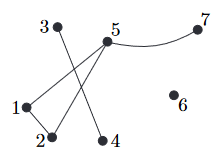
\includegraphics[width=0.5\linewidth]{graph_drawn.png}
    \caption[An~example of~graph visualization]{~An~example of~graph visualization~\cite{Diestel}.}
    \label{fig:graph_visualization}
\end{figure}
\section{Subgraph and Induced Subgraph}

When looking at~\autoref{fig:graph_visualization}, we can notice that the~\textit{sub-parts} of~the~graph can be considered graphs as~well. This leads us to~an~idea of~a~\textit{subgraph}.

\begin{definition}[Subgraph]
    Given two graphs $G = (V, E)$ and $H = (U, F)$. We say $H$ is a~\emph{subgraph} of~$G$ if $U \subseteq V$ and $F \subseteq E$.
\end{definition}
If $H$ is a~subgraph of~$G$, we can, slightly more informally, say that $G$ \textit{contains} $H$. Furthermore, if $H$ is a~subgraph of~$G$, we symmetrically say that $G$ is a~\textit{supergraph} of~$H$. \\
Apart from the subgraph we also define an~\emph{induced~subgraph}.
\begin{definition}[Induced subgraph]
    Given two graphs G = (V, E) and H = (U, F), we say H is an \emph{induced subgraph} of H if $U \subseteq V$ and $F = E \cap {U\choose2}$.
\end{definition}
The~difference between the~subgraph and~the~induced subgraph is that the~subgraph can contain any edges from~its supergraph. On~the~other hand, the~induced subgraph must include all edges existing in~its supergraph among the vertices it contains.

\section{Graph Families and Named Graphs}
In~this section, we are going to~look at~some usual graphs and~\textit{graph~patterns}. Typically, we are talking about a~graph with~a~stand-out structure, or a~graph that may represent a~shape well-known and common in~the~real world. One of~our main focuses will be to~describe the~relationships of graphs studied by~us and~these typical patterns.
\\
\\
\\

\subsection{Path}
\begin{definition}[Path]
    A~\emph{path} is a~non-empty graph $P = (V, E)$ such that: \\ $V = \{x_1, x_2, \dots, x_n\}, E = \{\{x_1, x_2\},\,\{x_2, x_3\},\,\dots,\,\{x_{n-1}, x_n\}\}$.
\end{definition}
A path is a~graph resembling a~route or~a~way between~two points. The~vertices contained in~only one edge (in~definition named as~$x_1$ and~$x_n$) are typically referred to~as~the~endpoints of~the~path.
An~important concept for~us is whether two points in~any graph are \textit{connected} by~a~path. Meaning whether there exists a~subgraph of~such graph, which is a~path with~the~two mentioned vertices being its endpoints. More formally, we define an~\emph{$s$,$t$-path}.
\begin{definition}[$s$,$t$-path]
    Let $G = (V, E)$ be a~graph and $s,t \in V$ be two vertices (source, target). An \emph{s,t-path} is a sequence $P = (v_1, v_2, \dots, v_l)$ such that $v_1 = s$, $v_l = t$; each vertex $v_i \in V$ appears in P at most once, and $\{v_i, v_{i + 1}\} \in E$ for every $1 \leq i \leq (l - 1)$.
\end{definition}
Both of~these concepts can be seen visualized in~\autoref{fig:paths}.

\begin{figure}
    \centering
    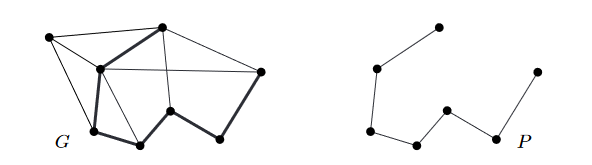
\includegraphics[width=1.0\linewidth]{path_example.png}
    \caption[An~example of~a~path subgraph and~a~path]{~An~example of~a~path subgraph~(left) and~a~path~(right)~\cite{Diestel}}
    \label{fig:paths}
\end{figure}

\subsection{Connected Graph}
A~graph is called \textit{connected}, if there exists a~path between any pair of~its vertices. More formally:
\begin{definition}[Connected graph]
    A~graph $G = (V,~E)$ is called \emph{connected} if there exists an~$s$,$t$-path for~all $s$,$t \in V$.
\end{definition}
A~graph which is not connected, is called \textit{disconnected}. Such graph consists of multiple \textit{connected components}.
\begin{definition}[Connected component]
    A~\emph{connected~component} is a~connected subgraph of graph that is not a~part of any larger connected subgraph.
\end{definition}
All connected components of~a~graph are disjoint and~together they add up to~the~whole graph.
\subsection{Cycle}
\begin{definition}[Cycle]
    A~\emph{cycle} is a~graph $C~=~(V,~E)$ of~pattern: \\ $V = \{x_1,\,x_2,\,\dots,\,x_n\}, E = \{\{x_1, x_2\},\,\{x_2, x_3\},\,\dots,\,\{x_{n-1}, x_n\},\,\{x_n, x_1\}\}$ where $n \geq 3$.
\end{definition}
A~cycle is a~typical graph resembling a~closed shape. We can notice that cycle is very similar to path, just with an~edge added between the~endpoints. Visualization of~a~cycle and~the~existence of~a~cycle as~a~subgraph in~a~graph can be seen in~\autoref{fig:cycles_visualization}.
\\
\\
\\
\subsection{Trees and Forests}
What is equally, if not more, important for~us is the~concept of~a~graph containing or~not containing a~cycle as~its subgraph.
\begin{definition}[Forest]
    A~graph is called a~\emph{forest} if none of~its subgraphs is a~cycle.
\end{definition}
We will often refer to~forests as~\textit{acyclic graphs}, due to~their characteristic of~not containing a~cycle. Furthermore, we define a~tree.
\label{TreeDefinition}
\begin{definition}[Tree]
    A~graph is called a~\emph{tree} if none of~its subgraphs is a~cycle and it is a~connected graph.
\end{definition}
As~we can see, every tree is a~forest with an~additional property of~existence of~a~path between~any pair of~its vertices.
\begin{figure}[h]
    \centering
    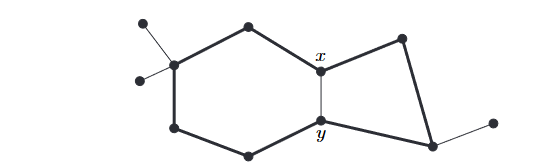
\includegraphics[width=0.75\linewidth]{cycle_example.png}
    \caption[An~example of~a~cycle as~a~subgraph of a~graph]{~An~example of~a~cycle~(bold) as~a~subgraph of a~graph~\cite{Diestel}.}
    \label{fig:cycles_visualization}
\end{figure}
\\
The terminology of~trees and~forests becomes more clear and~natural with~a~remark, that a~forest consists of~multiple connected components, in~which the~additional property holds. These components inherit the~property of~not containing cycles, making them trees. Therefore a~forest consists of~multiple trees and~a~tree is a~forest of~a~single tree.
Multiple definitions of~a~tree exist, all of~them describing the~same set of~graphs.
One of~these alternative definitions is:
\begin{definition}[Tree]
    A~graph G = (V, E) is called a~tree if it is a~connected graph and $|V| = |E| - 1$.
\end{definition}
Both definitions and their equivalency are shown in~the~monograph of~Diestel~\cite{Diestel}. \\
An~example of~visualization of~a~tree can be seen in~\autoref{fig:tree_visualization}.
\begin{figure}[h]
    \centering
    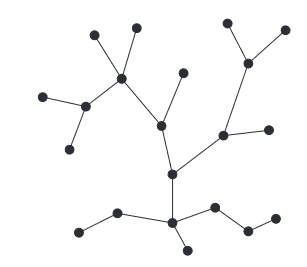
\includegraphics[width=0.5\linewidth]{tree_example.png}
    \caption[An example of a tree]{~An example of a tree~\cite{Diestel}.}
    \label{fig:tree_visualization}
\end{figure}

\subsubsection{Spanning Trees and Forests}
A~\textit{spanning}~subgraph is a~subgraph that contains all vertices of~its supergraph. A~spanning tree is a~subgraph which is a~tree.
\begin{definition}[Spanning tree]
    A~\emph{spanning tree} of~graph $G = (V, E)$ is a~subgraph ${T = (V, E')}$, where $E' \subseteq E$ and $T$ is a~tree.
\end{definition}
Existence of~a~spanning~tree requires the existence of a~path between any two vertices in~the~original graph. We can notice that a~graph for~which this property holds, can have more than one spanning~tree. \\
Very similarly, we can define the~spanning~forest as~a~forest containing all vertices of~its supergraph. Spanning~forests do not have any special requirements for~the~original graph. We can find a~spanning forest of any graph, and, once again, for~a~graph, multiple spanning~forests may exist.
\begin{definition}[Spanning forest]
    A~\emph{spanning~forest} of~graph $G = (V, E)$ is defined as~a~subgraph $F = (V, E')$, where $E' \subseteq E$, $F$ is a~forest and for~any two vertices holds, that if they were connected by~a~path in~$G$, then they are also connected by~a~path in~$F$. 
\end{definition}

\subsection{Petersen Graph}
\label{subsec:petersen}
Petersen graph is an~interesting example of~a~graph. It was constructed in~\cite{Petersen} by Danish mathematician Julius~Petersen, after~whom it is named. Over~the~years, it has proven to~be a~typical counter-example for~various propositions. In~the~next section, we are going to~define many graph properties. For better explanation, we are going to~demonstrate their value and~the~calculation procedure on~this particular example.
\\
\\
\begin{definition}
    Petersen graph is a~graph
    \[
        G = (
        V = \{u_0, \dots, u_4\} \cup \{v_0, \dots, v_4\},
        E = \{\{u_i, u_{i+1\,mod\,5}\}\, \{v_i, v_{i+2\,mod\,5}\}, \{u_i, v_i\} \mid 0 \leq i \leq 4\}
    \]
\end{definition}
The~visualization of~this graph can be seen in~\autoref{fig:petersen_visualization}.
\begin{figure}[h]
    \centering
    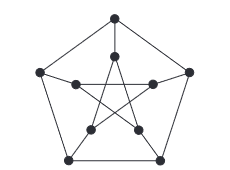
\includegraphics[width=0.5\linewidth]{petersen_original.png}
    \caption[Petersen graph]{~Petersen graph~\cite{Diestel}.}
    \label{fig:petersen_visualization}
\end{figure}

\section{Graph Properties}
We can define graph properties. Functions returning a~value for any graph on~which the~property is defined.

\subsection{Resemblance of a Tree/Forest}
As~we have declared previously, one of~the~focuses of~our interest will be measuring the~\textit{distance} of~a~studied graphs to~some of~the~particular graphs or~members of~graph~families mentioned earlier. In this section, we define a~few graph~properties, stating how~closely a~graph resembles a~tree~or~a~forest.

\subsubsection{Feedback Edge Set Number}
\label{subsubsec:fesn}
\textit{Feedback~edge~set~number} is a~property assigning any graph a~numerical value equal to~the~minimum number of~edges that have to~be removed from a~graph to~create a~forest (graph not containing any cycles).
More formally, we define \textit{the~feedback~edge~set} as~follows.
\begin{definition}[Feedback edge set~\cite{Beineke}]
    For a~given graph $G = (V, E)$, we define the~\emph{feedback~edge~set}, as~$F \subseteq E$ where~$G' = (V, E \setminus F)$ is a~forest.
\end{definition}
Now, we can continue with~defining the~\textit{feedback~edge~set~number}.
\begin{definition}[Feedback edge set number]
    We define the~\emph{feedback~edge~set~number}, denoted FESN, of~a~graph~$G$ as~the~smallest possible cardinality of~$F$ across~all possible feedback~edge~sets of~a~graph~$G$.
\end{definition}
For~better explanation, let us take the~famous Petersen~graph and~demonstrate the~value of~this property on~this example. The~Petersen~graph has the~feedback edge~set~number equal to~6. As~there are 6 edges that can be removed in~order to~create an~acyclic graph, and~there are no~such 5~(or~less) edges that would make the~graph acyclic after~their removal. To~discover this value, we first identify any spanning tree (or~forest for a~disconnected graph) of~the graph, which is the~maximal acyclic subgraph, and~then take the~remaining edges as~the~feedback~edge~set. The~calculation procedure can be better seen in~\autoref{fig:fesn_petersen_2}.
The~black edges are the~6 edges that have to~be removed, the~remaining red edges form~a~spanning~tree. We can see that if we would add any of~the~black edges to~the~graph, then the~graph would contain a~cycle. The~black edge connects two vertices between which $s,t$-path surely exists (because the spanning tree is connected). This $s,t$-path, together with the~added black edge would form a~cycle. Therefore, the~feedback~edge~set number can not be~5 or~lower, as removing 5 edges will surely leave a cycle in the graph. For~better description of~the~computation of~feedback edge set number for~Petersen graph and~other graphs, please refer to~\cite{Beineke}.
\pagebreak
\begin{figure}
    \centering

        \begin{tikzpicture}[every node/.style={draw,circle,very thick}]
          \graph[clockwise, radius=2cm] {subgraph C_n [n=5,name=A] };
          \graph[clockwise, radius=1cm] {subgraph I_n [n=5,name=B] };
        
          \foreach \i [evaluate={\j=int(mod(\i+2+4,5)+1)}]% using Paul Gaborit's optimisation
             in {1,2,3,4,5}{
            \draw (A \i) -- (B \i);
            \draw (B \j) -- (B \i);
            \draw[red] (A 1) -- (B 1);
            \draw[red] (A 1) -- (A 2);
            \draw[red] (A 1) -- (A 5);
            \draw[red] (B 1) -- (B 3);
            \draw[red] (B 1) -- (B 4);
            \draw[red] (A 2) -- (B 2);
            \draw[red] (A 2) -- (A 3);
            \draw[red] (A 5) -- (B 5);
            \draw[red] (A 5) -- (A 4);
          }
        \end{tikzpicture}
        \caption[Petersen graph with the spanning tree and the feedback edge set marked]{~Petersen graph with the spanning tree (red) and the feedback edge set (black) marked, taken from \cite{soPetersen}, modified.}
        \label{fig:fesn_petersen_2}
\end{figure}

% We could have also calculated feedback edge set number as 6 just from the knowledge of sizes of vertices (10) and edges (15) as we have demonstrated in the calculation part. The minimum spanning tree of this graph will have size 9 (one less then the number of vertices), therefore the Feedback Edge Set Number will be surely 6, because it has to be equal to the size of edges minus the size of minimum spanning tree.
\subsubsection{Feedback Vertex Set Number}
\label{subsubsec:FeedbackVertexSetNumber}
Very similar in~terms of~definition, but, as~we will discuss later, very different in~terms of~complexity of~computation, is the~\textit{feedback~vertex~set~number}.
Feedback~vertex~set~number is a~property assigning any graph a~numerical value equal to~the~minimum number of~vertices that have to~be removed from a~graph to~create an~acyclic graph~(a~forest). \\
First, we define the~\textit{feedback~vertex~set}.
\begin{definition}[Feedback vertex set \cite{Beineke}]
    For~a~given graph $G = (V, E)$, we define the~\emph{feedback~vertex~set}, as~$F \subseteq V$ where~$G' = (V \setminus F, E)$ is a~forest.
\end{definition}
Or~equivalently:
\begin{definition}[Feedback vertex set]
    We can also define the~\emph{feedback~vertex~set} for~a~given graph~$G = (V, E)$, as~$F \subseteq V$, where~vertices of~every cycle contained in~$G$ have a~non-empty intersection with~$F$.
\end{definition}
These two definitions are equivalent. If we hold a~set of~vertices that includes at~least one vertex from~every cycle, then removing these vertices will break all the~cycles, as~the~cycles will disconnect on~the~removed vertex. \\
If we would have a~set of~vertices that does not include any vertex from~at~least one of~the~cycles in~the~graph, then such set will not make the~graph acyclic after~removal, as~the~cycle not~\textit{hit} by~the chosen vertices subset, will remain present after~the~removal of~this subset.\\
Now, we proceed to~defining the~\textit{feedback~vertex~set~number}.
\begin{definition}[Feedback vertex set number]
    We define the~\emph{feedback~vertex~set~number}, denoted FVSN, of~a~graph~$G$ as~the~smallest possible cardinality of~$F$ across all possible feedback~vertex~sets of~graph~$G$.
\end{definition}
Let us demonstrate the~property once again at~the~notorious Petersen~graph.
\begin{figure}
    \centering
        \begin{tikzpicture}[every node/.style={draw,circle,very thick}]
          \graph[clockwise, radius=2cm] {subgraph C_n [n=5,name=A] };
          \graph[clockwise, radius=1cm] {subgraph I_n [n=5,name=B] };
        
          \foreach \i [evaluate={\j=int(mod(\i+2+4,5)+1)}]% using Paul Gaborit's optimisation
             in {1,2,3,4,5}{
            \draw (A \i) -- (B \i);
            \draw (B \j) -- (B \i);
          }
        \end{tikzpicture}
            \begin{tikzpicture}[every node/.style={draw,circle,very thick}]
                \graph[clockwise, radius=2cm] {subgraph C_n [n=5,name=A] };
                \graph[clockwise, radius=1cm] {subgraph I_n [n=5,name=B] };
            
                \foreach \i [evaluate={\j=int(mod(\i+2+4,5)+1)}] in {1,2,3,4,5}{
                    \draw (A \i) -- (B \i);
                    \draw (B \j) -- (B \i);
                }
                \node[draw,circle,very thick,red] at (A 5) {5};
                \node[draw,circle,very thick,red] at (B 3) {3};
                \node[draw,circle,very thick,red] at (B 4) {4};
            \end{tikzpicture}
            \begin{tikzpicture}[every node/.style={draw,circle,very thick}]
                \graph[clockwise, radius=2cm] {subgraph C_n [n=5,name=A] };
                \graph[clockwise, radius=1cm] {subgraph I_n [n=5,name=B] };
            
                \foreach \i [evaluate={\j=int(mod(\i+2+4,5)+1)}] in {1,2,3,4,5}{
                    \draw (A \i) -- (B \i);
                    \draw (B \j) -- (B \i);
                }
                \node[draw,circle,very thick,white] at (A 5) {5};
                \node[draw,circle,very thick,white] at (B 3) {3};
                \node[draw,circle,very thick,white] at (B 4) {4};
            
                \draw[white] (A 1) -- (A 5);
                \draw[white] (A 4) -- (A 5);
                \draw[white] (B 5) -- (A 5);
                \draw[white] (A 4) -- (B 4);
                \draw[white] (B 1) -- (B 4);
                \draw[white] (B 2) -- (B 4);
                \draw[white] (B 1) -- (B 3);
                \draw[white] (B 5) -- (B 3);
            \end{tikzpicture}
            \caption[Petersen graph with the feedback vertex set marked and removed]{Petersen graph~(left) with the feedback vertex set marked in red~(middle)\\ and removed~(right), taken from \cite{soPetersen}, modified.}
        \label{fig:fvsn_petersen_2}
    \end{figure}
First, we show that Petersen graph has a~feedback~vertex~set of size 3. That can be seen in \autoref{fig:fvsn_petersen_2}. In~the~second picture, the~red vertices are the~ones marked for~removal. In~the~third picture, we can see that the~graph is acyclic, after~the~marked vertices have been removed. Note that there are multiple possibilities how~to~choose such~3~vertices. For example, choosing an~outer~2, instead of~outer~5, would work as~well. \\
Now, we show that there can not exist a~feedback~vertex~set of~size~2. We surely have to~break the~inner and the~outer cycle, so the~2~selected vertices must be from~the~different parts of~the~graph. Let us consider without loss of~generality that we select vertex number~1 from the~outer cycle (for~any other vertex, the~situation would be identical, the~numbers would only~slightly shift).
Removing vertex 1, 3, or~4 from the~inner cycle, would leave us with~cycle~5-5-2-2-3-4 and~removing vertex~2 or~5, would leave us with~cycle~1-1-3-3-2~\cite{Beineke}.
\subsubsection{Treewidth}
\label{subsubsec:treewidth}
The treewidth is another numerical property describing how~distant is the~graph in~question to~a~tree. The~distance in~this case is not so~straight-forward to~see like in~the~case of~feedback~set~numbers. The treewidth describes rather how~close is the~graph to~being a~tree when processing the~graph algorithmically. This makes the~treewidth a~very useful parameter for~further processing of~the~graph, as~many computations can be simplified, when the~treewidth~of~a~graph is known, especially, when the~treewidth is low.~\cite{Diestel} \\
Let us start with~the~definition of~a~\textit{tree~decomposition}, which is a~crucial concept for~the~definition of~the~treewidth.
\begin{definition}[Tree decomposition]
Given a~graph $G~=~(V,~E)$, we define its \emph{tree~decomposition} as~a~triple $T = (V_T, E_T, \beta)$, where $\beta: V_T \rightarrow 2^V \setminus \{\emptyset\}$. For~better clarity, we will refer to~elements of~$V$ as~vertices and~elements of~$V_T$ as~nodes. $\beta$ is a~map mapping nodes of~$V_T$ onto subsets of~vertices of~$V$. These subsets must satisfy three conditions.
\begin{samepage}
    \begin{itemize}
        \item $\bigcup_{x \in V_T} \beta(x) = V$;
        \item for~every edge~$\{u, v\}\in E$ there exists a~node~$n \in V_T$, such that $u \in \beta(n) \land v \in \beta(n)$;
        \item for every vertex ${v \in V}$, a subgraph $T'$ of $T$, such that\\
        ${T' = (\{x \mid x \in V_T \land v \in \beta(x)\}, \{\{x, y\}\ \mid v \in \beta(x) \land v \in \beta(y) \land \{x, y\} \in E_T\})}$ is a~tree.
    \end{itemize}
\end{samepage}
     The~graph defined as~$(V_T, E_T)$ must form a~tree.
\end{definition}
To~put this rather complicated definition into~a~natural language. We construct a~tree with~nodes being the~subsets of~vertices of~the~original graph. There are three conditions on~these subsets.
The first item of~the~three tells us that every vertex from~$V$ has to~be included in at~least one subset from~$V_T$. \\
The~second condition tells us, that if there are two vertices directly connected by~an~edge in~graph~$G$, then there necessarily must exist a~subset in~$V_T$ containing both of~them.\\
The~last required property of~the~tree~decomposition is~the~tree-ness of~subgraphs~of~$T$ induced by~vertices from~$V$. If we take a~vertex from~$V$, and~then look at~subgraph of~$V_T$ that includes only nodes containing the~selected vertex and edges between these nodes, we must get a~tree. This must hold for~all vertices from~$V$.
Now, we can continue with~the~definition of~width of~a~tree~decomposition and~treewidth of~a~graph.
\begin{definition}[Treewidth]
     A~width of~a~tree~decomposition~${T = (V_T, E_T, \beta)}$ is equal to~${\max_{v \in V_T} | \beta(v) | - 1}$. \\
    A \emph{treewidth} of~a~graph is equal to~the~smallest possible width across all possible tree~decompositions of~this graph.
\end{definition}
Let us demonstrate the~treewidth on~the~Petersen~graph. The~minimal tree~decomposition~(in terms of~its treewidth) can be seen in. \\
This decomposition is a~valid tree decomposition, as the~graph is clearly a~tree~(does not contain any cycle and is connected) and all three required conditions are met. The~first property holds, as every number is present in at~least one node of~the~decomposition. The second condition also holds. The~vertex labeled by 0 in the~original graph is connected by an edge with vertices 1, 4 and~5. Therefore in~the~tree decomposition, we can identify a~node containing 0~and~1, and~another node~(could be also the~same node) containing 0~and~4, and another node containing 0~and~5. This holds for any vertex in the original graph. The last required property also holds. If we take the~subgraph of the~tree decomposition induced by nodes containing vertex labeled with~2 in the original graph, we get the~two~bottom-right vertices. These vertices are connected and acyclic, thus they form a tree. This once again holds for all vertices from the~original graph. Therefore the shown graph is a valid tree decomposition. The proof that we can not find a tree decomposition with smaller width is shown in \cite{Huszár}.
Therefore the treewidth of~Petersen~graph is equal to~4.
\begin{figure}[h]
\centering
\begin{tikzpicture}[every node/.style={draw,circle,very thick}]
  \graph [clockwise,math nodes] {
    subgraph C_n [V={0,1,2,3,4},name=A, radius=2cm]; 
    subgraph I_n [V={5,6,7,8,9},name=B, radius=1cm];
    }; 
    \draw (B 6) -- (A 1);
    \draw (B 7) -- (A 2);
    \draw (B 8) -- (A 3);
    \draw (B 9) -- (A 4);
    \draw (B 5) -- (A 0);
    \draw (B 7) -- (B 5);
    \draw (B 9) -- (B 7);
    \draw (B 6) -- (B 9);
    \draw (B 8) -- (B 6);
    \draw (B 5) -- (B 8);
\end{tikzpicture}  


    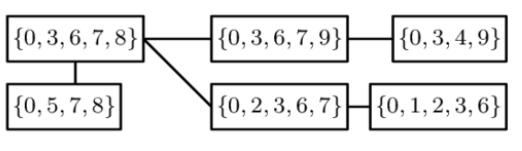
\includegraphics[width=0.5\linewidth]{petersen_tree_decomposition.png}
    \caption[A~tree~decomposition of~Petersen~graph]{~A~tree~decomposition of~Petersen~graph,~\cite{Huszár}.}
    \label{fig:td_petersen_2}
\end{figure}
\subsection{Graph Covering Numbers}
Coverings problems typically refer to~taking a~part of~a~graph, which, in~a~certain way, \textit{covers} the~whole graph. \\
The~graph properties of~graph covering numbers typically refer to~numerically expressing the~minimal~covering of~the~graph.
\subsubsection{Vertex Cover Number}
\label{subsubsec:VCN}
\textit{Vertex cover} is a~set of~vertices, such that every edge contains at~least one vertex of~this subset.
\begin{definition}[Vertex cover~\cite{Garey}]
    Given a graph $G = (V, E)$, we say that a~subset of~vertices ${F \subseteq V}$ is a~\emph{vertex~cover} if ${\,\forall \{u, v\} \in E: u \in F \lor v \in F}$
\end{definition}
Then we define the~\textit{vertex~cover~number} as~the~smallest possible vertex~cover for~a~graph.
\begin{definition}[Vertex Cover Number]
    We define \emph{vertex~cover~number} of~a~graph~$G$ as~a~smallest possible cardinality across all vertex~covers of~the~graph~$G$.
\end{definition}

\begin{center}
    \begin{figure}[h!]
        \centering
            \begin{tikzpicture}[every node/.style={draw,circle,very thick}]
                \graph[clockwise, radius=2cm] {subgraph C_n [n=5,name=A] };
                \graph[clockwise, radius=1cm] {subgraph I_n [n=5,name=B] };
            
                \foreach \i [evaluate={\j=int(mod(\i+2+4,5)+1)}] in {1,2,3,4,5}{
                    \draw (A \i) -- (B \i);
                    \draw (B \j) -- (B \i);
                }
                \node[draw,circle,very thick,red] at (A 1) {1};
                \node[draw,circle,very thick,red] at (A 2) {2};
                \node[draw,circle,very thick,red] at (A 4) {4};

                \node[draw,circle,very thick,red] at (B 3) {3};
                \node[draw,circle,very thick,red] at (B 4) {4};
                \node[draw,circle,very thick,red] at (B 5) {5};
            \end{tikzpicture}
        \caption[Petersen~graph with the optimal vertex cover]{~Petersen~graph with the~optimal vertex cover highlighted in~red, taken from~\cite{soPetersen}, modified.}
        \label{fig:vc_petersen}
    \end{figure}
\end{center}
For~better clarity, we are going to~once again demonstrate this property on~Petersen~graph.
Petersen~graph has the~vertex~cover~number equal to~6. First, we show that there exists a~set of~6~vertices that covers all edges of~the~graph. Such cover can be seen in~\autoref{fig:vc_petersen}. Next we show that we can not identify a~set of~size~5~(or~smaller) that would cover the whole graph. We can see that every vertex in~the~Petersen~graph is incident with~exactly 3~edges. Therefore, any vertex added to~the cover, can add at~most~3 covered edges. Since the graph has 15~edges, there can not exist a~vertex cover of~size~4 or~smaller, because 4~vertices could only cover at most 12~edges. Should there exist a~vertex cover of~size~5, than necessarily, each vertex must add all of~its 3~incident edges to~the~set of~covered edges. Meaning that each incident edge must not have been added previously to~the~set by any other vertex in the cover. This implies that the~5~selected vertices must not share a~common edge\footnote{In other words, they must form an~independent set.}. Now we show that such 5~vertices can not be found in this graph. The~graph consists of two cycles of~length~5. Once we select 2~vertices from a cycle of length~5, we can not find any other vertex in~the~cycle that would be connected to neither of selected. Once we select two vertices from the~outer cycle and two vertices from the inner~cycle, we can not find any other vertex in~the graph that would not be incident with the~selected vertices. Thus we can not find 5~vertices not sharing a~common edge, which means that there can not exist a~vertex cover of~size~5. The~calculation of~the~vertex~cover~number of~Petersen~graph is better explained in~\cite{Behsaz}.
\subsubsection{Edge Cover Number}
\label{subsubsec:EdgeCoverNumber}
\textit{Edge~cover~number} also refers to~minimal covering of~a~graph, but this time using its edges.\\
We once again start with defining the~covering~set. \textit{Edge~cover} is a~subset of~edges, such that for~every vertex, there is an~edge in~the~subset, containing it.
\begin{definition}[Edge cover~\cite{Garey}]
    Given a~graph ${G = (V, E)}$ we say that a subset of~edges~${F \subseteq E}$ is an \emph{edge cover} if: ${\,\forall v \in V: \exists e \in E: e \in F \land v \in e}$
\end{definition}
We then proceed to~define the~\textit{edge~cover~number} very similarly as~the~vertex~cover~number.
\begin{definition}[Edge cover number]
    We define the~\emph{edge~cover~number} of~a~graph~$G$ as~the~smallest possible cardinality across all edge~covers of~the~graph~$G$.
\end{definition}
\begin{remark}
    Smallest possible edge~cover~number for~a~graph of~$n$~vertices is~${\lceil\frac{n}{2}\rceil}$, as every edge selected into~cover is incident with~exactly 2~vertices. Therefore a~single edge can add at~most 2~covered vertices. Assuming there exists an~edge~cover of~size~${\lceil\frac{n}{2}\rceil - 1}$ or smaller, would necessarily mean that such edge~cover covers~at~most ${n - 1}$ vertices, which is a~contradiction with~the~edge~cover covering all $n$~vertices in~the~graph.
\end{remark}
For~better clarity, we are going to~once again demonstrate this property on~Petersen~graph. \\
An~optimal edge~cover for Petersen~graph is not hard to~find. We can simply take the~edges connecting the~outside cycle and~the~inner cycle. Such edge~cover has cardinality~5. Since the~Petersen~graph has 10~vertices, we can not find a~smaller edge cover~(according to~the~previous remark); therefore the~edge cover~number of~Petersen~graph is~5. The~cover can be seen in~\autoref{fig:ec_petersen}
\begin{center}
    \begin{figure}[h!]
        \centering
            \begin{tikzpicture}[every node/.style={draw,circle,very thick}]
                \graph[clockwise, radius=2cm] {subgraph C_n [n=5,name=A] };
                \graph[clockwise, radius=1cm] {subgraph I_n [n=5,name=B] };
            
                \foreach \i [evaluate={\j=int(mod(\i+2+4,5)+1)}] in {1,2,3,4,5}{
                    \draw[red] (A \i) -- (B \i);
                    \draw (B \j) -- (B \i);
                }
            \end{tikzpicture}
        \caption[Petersen graph with the~optimal edge cover]{~Petersen graph with the optimal edge cover highlighted in red, taken from \cite{soPetersen}, modified.}
        \label{fig:ec_petersen}
    \end{figure}
\end{center}

\chapter{Computational Complexity}
In~this chapter, we are going to~discuss theory of~computational~complexity. Throughout this thesis, we are going to~stumble upon many \textit{NP-hard} problems, this chapter gives an~explanation, why we have not tried to~design an~efficient algorithm for~these problems, and~rather opted to~use existing solvers. Although designing an~efficient algorithm for~these problems is not deemed impossible the~question whether such algorithm can exist, is the~central undisclosed topic of~computer~science unsolved for~long years. \\
To~keep this chapter brief, we are going to~limit ourselves only on~the~P and~NP complexity~classes and~the~related sets of~problems. For~more information about this topic please refer to~the~monograph of~Arora~and~Barak~\cite{Arora}.
\section{Input Encoding}
In~this section, we briefly mention unification of~input formats by~encoding inputs into a~string.
First we start by~defining few basic concepts of~language theory.
\begin{definition}[Alphabet]
    An \emph{alphabet} is a~finite non-empty~set of~characters.
\end{definition}
\begin{definition}[String]
    A~\emph{string} over an~alphabet is a~finite sequence of~characters of~the~alphabet.
\end{definition}
\begin{definition}[Language]
    \emph{Language}~$L$ over the~given alphabet $A$ is a~subset of~all possible strings of~$A$.
\end{definition}
Our typical alphabet will be binary $\{0, 1\}$, as~all the~assumed inputs can be encoded as binary strings. When we say that a~certain problem has two numbers on~the~input, we actually mean that on input it has a~binary~string with~these numbers encoded. We are not going to~let distract ourselves with the~low level details of encoding, as they are not the~main object of~our study, and focus on~the~bigger picture.
\section{Decision Problem}
In~a~\textit{decision~problem}, our goal is to~decide whether given input satisfies a~certain condition. More formally:
\begin{definition}
    A~\emph{decision~problem} is a~language $L = \{x \mid f(x) = 1\}$, where $f$ is a~function mapping a string onto 0 or 1, depending on~whether the~string satisfies a~specified condition.
\end{definition}
\section{Computation}
\textit{Computation} is the~process of~determining the~value of~the~function for~given input. The~computation process generally consists of~following steps:
\begin{itemize}
    \item read a~character from input;
    \item read a~character from~inner memory;
    \item write a~character into inner memory;
    \item either stop outputting a~character, or~pick a~new rule that will be applied next in~the~computation process.
\end{itemize}
\section{Turing Machines}
We are going to~use the~computation~model of \textit{Turing~machine} as~described by~Alan~Turing~\cite{Turing}.
\subsection{$k$-tape Turing Machine}
The~inner memory of a~$k$-tape~Turing~machine consists of~$k$~tapes, with the~tape being an~infinite line of~memory cells, which can hold a~symbol of~working alphabet of~the~machine. \\
All tapes have their own \textit{head}. In~every step of~the~computation, the~head can read symbol from~its current~cell, write a~symbol into~the~current~cell, and/or~change the~current~cell by~moving left or~right. \\
The~first tape is considered the~\textit{input~tape}, containing the~input of~the~problem. It is \textit{read-only}, meaning that its head is not capable of~writing characters into~memory~cells. \\
The~last tape is considered the~\textit{output~tape}. The~output of computation is present on~the~output tape, when the~Turing~machine \textit{halts}.\\
The~remaining tapes are considered the~\textit{working~tapes}.
\subsection{Deterministic $k$-tape Turing Machine}
Let us move to~defining the~computation model of~a~deterministic variant of~the~Turing~machine.
\begin{definition}[Deterministic k-tape Turing machine]
    A \emph{deterministic~$k$-tape~Turing~machine} is a~tuple~${TS = (A, Q, \delta)}$, where
    \begin{itemize}
        \item $A$ is~the~alphabet of~the~machine containing two special symbols. One of them being a~blank symbol $\square \in A$ and the~other being the~start symbol $\triangleright \in A$;
        \item $Q$ is the~set of~states of~the~machine, with one state $q_0 \in Q$ being the~start state and one state $q_{halt} \in Q$ being the~halting state;
        \item $\delta$ is a~function~${Q \times A^k \rightarrow Q \times A^{k-1} \times \{L, S, R\}^k}$ called the~transition function.
    \end{itemize}
\end{definition}

\subsection{Non-deterministic $k$-tape Turing Machine}
Now we will define the~non-deterministic counterpart of~this computation~model.
\begin{definition}[Non-deterministic $k$-tape Turing machine]
    A~\emph{non-deterministic~$k$-tape~Turing~machine} is a~tuple~${TS = (A, Q, \delta)}$, where
    \begin{itemize}
        \item $A$ is the~alphabet of~the~machine containing two special symbols. One of them being a~blank symbol $\square \in A$ and the~other being the~start symbol $\triangleright \in A$;
        \item $Q$ is the~set of~states of~the~machine, with~two special states. One of~them being again the~start state $q_0 \in Q$, and~the~other being the~accept state $q_{accept} \in Q$.
        \item $\delta$ is a function ${Q \times A^k \rightarrow 2^{Q \times A^{k-1} \times \{L, S, R\}^k}}$ called the~transition function.
    \end{itemize}
\end{definition}

\subsection{Computation of Turing Machines}
The~transition function has on its input a~state the~machine is currently in, and~$k$~characters, read by~all $k$~heads. For~such input, it returns a~new state, in~which the~machine will be now; $k - 1$ characters to~write by all heads (except for~the~input~tape one), and a~command \textit{Left}, \textit{Stay}, or~\textit{Right} for~all $k$~heads to~change their current cell. \\
At~the~beginning of~the~computation, all tapes are filled with~the~blank symbol~$\square$, except for~the~input tape. Input tape contains a~start symbol~$\triangleright$ followed by~the~finite input string. The~rest of~the~input~tape is initialized with the~blank symbol, just like the~other tapes.\\
The~initial state of~the~machine is the~start state~$q_0$. The~machine then applies the~transition function as~explained above, until it reaches the~halting state. After the~Turing~machine reaches its halting state, it halts and the~contents of~the~tapes are not modified further. It is also possible for a certain input that the~Turing machine may never reach the~halting state, in that case the Turing~machine never halts, therefore it does not accept the~input.
\subsubsection{Computation of Non-deterministic Turing Machines}
In~the~non-deterministic variant of~the~Turing~machine the transition function returns the same instructions as~the~deterministic variant~(new state, characters to~write, commands for heads), however the function returns a~set of possibilities. In every step the non-deterministic Turing~machine makes an~additional decision which of~these possibilities to~use. If there exists a~sequence of~these decisions that gets the~Turing~machine into~the~state of~$q_{accept}$, then the~result of~the~computation is~1. If none of~the~decision sequences gets the~machine into~the~state of~$q_{accept}$, the~result of~the~computation is~0.

\section{Complexity Classes}
\label{sec:Complexity classes}
Now, with~the~computational models defined, we can define the~concept of~\textit{complexity~class} and~few particular complexity~classes.
\begin{definition}[Complexity class]
    \emph{Complexity~class} is a~set of decision~problems that can be computed with a~given complexity~resource.
\end{definition}
We are going to focus on complexity resource of \textit{running time}. Let us firstly formalize and define this complexity resource.
\begin{definition}[Running time]
    Let $f$ be a~decision~problem, $T$ be a~function~${\mathbb{N} \rightarrow \mathbb{N}}$, and~$M$~be a~Turing~machine. We say that $M$ computes $f$ in~$T(n)$~time, if for every string~$x$ it halts with~$f(x)$ on~output tape after~at~most $T(|x|)$~steps\footnote{Applications of transition function.}. 
\end{definition}
\pagebreak
\subsection{P Complexity Class}
Let us start with~the~definition of~the~complexity~classes of~\textit{DTIME}\footnote{DTIME stands for deterministic time.}.
\begin{definition}[DTIME]
    For a~function ${f : \mathbb{N} \rightarrow \mathbb{N}}$, we define DTIME(f(n)) as~a~set of~all decision~problems computable on~a~deterministic~Turing~machine in~$c \cdot f(n)$ time, for some constant~${c > 0}$.
\end{definition}
Now, we can define the~\textit{P}\footnote{P stands for polynomial} \textit{complexity class}.
\begin{definition}[P complexity class]
    $P = \bigcup_{c \geq 1}\text{DTIME}(n^c)$
\end{definition}
P~class consists of~all decision problems computable in~polynomial~time on~a~deterministic~Turing~machine. This can be vaguely translated as~\textit{problems that are efficiently computable in~our world}. We will often address problems contained in P as problems computable in polynomial time.
\subsection{NP Complexity Class}
Very similarly, we are going to define the~\textit{NP}\footnote{NP stands for non-deterministic polynomial} \textit{complexity class}. We will start with the~definition of~\textit{NTIME}\footnote{NTIME stands for non-deterministic time}, a~non-deterministic variation of~DTIME defined earlier.
\begin{definition}[NTIME]
    For a~function ${f : \mathbb{N} \rightarrow \mathbb{N}}$, we define NTIME(f(n)) as~a~set of all decision~problems computable on a~non-deterministic~Turing~machine in~${c \cdot f(n)}$ time, for some constant~${c > 0}$.
\end{definition}
Now we can define the~NP~complexity~class as follows:
\begin{definition}[NP complexity class]
    NP~=~$\bigcup_{c \geq 1}\text{NTIME}(n^c)$
\end{definition}
An~equivalent definition of~NP~class is the following:
\begin{definition}[NP complexity class]
    A~decision~problem~$f$ is a~member of~NP~class, if there exists a~polynomial $p: \mathbb{N} \rightarrow \mathbb{N}$ and~a~deterministic~Turing~machine~$TM$, such that for~every binary string~$x$:
    ${f(x) = 1 \iff \exists\,u \in \{0, 1\}^{p(|x|)} \text{, such that } TM(x, u) = 1}$, which can be computed in polynomial time.
\end{definition}
Proof of~equivalency of~these definitions can be seen in~\cite{Arora}.\\
This alternative definition tells us that for every input string $x$ exists a \textit{certificate} $u$ of polynomial length that \textit{certifies} the~fact that $x$ is an~element of~the~language. \\
To~see an~example of~such certificate, let us take the~decision problem of~whether a~given graph has a~feedback~vertex~set~(as defined in \autoref{subsubsec:FeedbackVertexSetNumber}) of~size~$k$. This problem is a~member of~NP~class. The~certificate in this case is a~list of~$k$~vertices that form a~feedback~vertex~set. Given such certificate, we could detect whether the~graph contains any cycle after removing the~vertices included in~the~list. Such problem is known to~be solvable in~polynomial time using depth-first~search~\cite{Diestel}.\\
The NP~class consists of~decision~problems that can be \textit{verified} in polynomial time on a~deterministic~Turing~machine. Given an~instance of~a~problem and~a~solution~(certificate), Turing~machine can verify that the~solution solves the~problem. \\
The~non-deterministic~Turing~machine can try all possible solutions in~its computational branches and if one of them is a~solution that certifies the~presence of~input in~language, then the~Turing~machine will reach $q_{accept}$ in~that computational branch, yielding the~output of~1. \\
If we let a non-deterministic~Turing~machine compute a problem from NP class, then the~non-deterministic decisions used for transition into~$q_{accept}$, made by~such Turing~machine, are also a~valid certificate for~the~input.
\subsection{NP-hardness and NP-completeness}
In this subsection, we are going to define the concepts of \textit{NP-hardness} and \textit{NP-completeness}.
We start by defining the \textit{polynomial reducibility} among decision problems.~\cite{Karp, Cook}
\begin{definition}[Polynomial-time reudcibility]
    We say that a~language~$A \subseteq L$ is \emph{polynomial-time reducible} to~a~language~$B \subseteq L$, where $L$ is set of~all binary strings; if there exists a~polynomial-time computable function $f: L \rightarrow L$, such that $\forall x \in L: x \in A \iff f(x) \in B$.
\end{definition}
We can see that if the problem~$A$ is polynomial reducible to~$B$, and we would be able to~compute~$B$ in polynomial time, then we would be able to~compute $A$ in~polynomial time. \\
Now we can move onto~definition of~an~\textit{NP-hard problem}.
\begin{definition}[NP-hardness]
    A~decision problem~$K$ is said to~be \emph{NP-hard} when for~every problem~$L$ in~NP there exists a~polynomial time reduction from~$L$ to~$K$
\end{definition}
Subsequently, we define the \textit{NP-complete} problems.
\begin{definition}[NP-completeness]
    A~decision~problem is said to~be \emph{NP-complete}, if it is NP-hard and it is a~member of~NP~class.
\end{definition}
\subsection{Relation of P and NP Complexity Classes}
Trivially, we can see that:
P $\subset$ NP. However, probably the~biggest undisclosed question of~computer~science is whether P~\textit{equals}~NP. Finding an~answer to~this question might be one of~the~biggest advances in~the~modern science. Thanks to~its importance, \textit{P versus NP problem} has been placed on~the~list of~Millenium Prize Problems~\cite{Jaffe}. \\
If P~would equal~NP, then all NP~problems would most probably be efficiently solvable in~our world. This equality could be proved by finding a~polynomial algorithm for any of~the~NP-hard problems. As~it would mean that all NP problems can be converted in~polynomial time to a~problem, solvable in~polynomial time. Therefore, solving NP-hard problems in~polynomial time is a~very ambitious task. In~this thesis we rather used existing solvers, which are able to~solve some NP-hard problems in~bearable time for smaller inputs using heuristics or~other techniques. \\
Solving NP-hard problems using heuristics is an~interesting discipline of~computer science. For example PACE\footnote{Parameterized Algorithms and Computational Experiments} holds every year an~annual competition, where a~particular NP-hard problem is selected and~the~competitors are trying to~design the~fastest program for~computation of~the~problem~\cite{PACE}. In~this thesis, we are going to~use for practical usage some of~the~algorithms submitted into~this competition.
\section{Notable NP-hard Problems}
In~this section we mention few NP-hard problems that we will discuss further in~our work. Definitions of~these problems and~a~proof of~NP-hardness, can be seen in~\cite{Diestel, Arora, Karp}.
Following problems are included in~the~set of~NP-hard problems:
\begin{itemize}
    \item the problem of whether graph contains a feedback vertex set of size $k$,
    \item the problem of whether there exists a tree decomposition of the given graph of width $k$,
    \item the problem of whether the given graph can be covered using $k$ vertices,
    \item the problem of finding the hitting set of size $k$,
    \item the problem of 0-1 integer programming.
\end{itemize}
The first three problems were introduced in the~first chapter. Let us introduce the other two.
\begin{definition}[The problem of finding the hitting set of size $k$]
    Given a~family of sets $F = \{S_1,\,S_2,\,\dots,\,S_n\}$, find a subset of size $k$ of~the~universum $A \subseteq \bigcup_{S \in F} S$, such that $\forall S \in F: A \cap S \neq \emptyset$.
\end{definition}
\begin{definition}[The problem of 0-1 integer programming]
    Given a~matrix~${A \in \mathbb{Z}^{m,n}}$ and~a~vector $b \in \mathbb{Z}^m$, determine, whether there exists a~vector~$x \in \{0, 1\}^n$, such that $Ax \leq b$\footnote{Using elementwise comparison.}.
\end{definition}

\chapter{Linear Programming}
\emph{Linear~programming} revolves around solving optimization problems in a~given mathematical model. Its origins date to~the~times of~Fourier and~it has been described long before invention of~the~modern computers; therefore it has been well studied by~mathematicians, economists, and~other scientists, and~grew to giant dimensions. We will only go~quickly through few topics related to~our work. For a~better overview of~the~whole topic, please refer to~\cite{Sierksma}.
\section{Linear Program}
The~\emph{linear~programming} is focused around optimizing a~linear objective function while respecting given linear equalities or~inequalities.\\
Linear program consists of
\begin{itemize}
    \item variables, typically denoted $x_1, \dots, x_n \in \mathbb{R}$;
    \item an objective function $c_1x_1 + \dots + c_nx_n$, where $c_1, \dots, c_n \in \mathbb{R}$, to be maximized or minimized;
    \item a set of constraints in form $a_1x_1 + \dots + a_nx_n\,(\geq | = | \leq)\,b$.
\end{itemize}
A~vector $x \in \mathbb{R}^n$ satisfying all constraints, is called a~\textit{feasible~point} or~a~\textit{feasible~solution}. The~set of~all feasible points is called the \textit{feasible region} of the model. If the model has an empty feasible region, then the model is called \textit{infeasible}. An~optimal solution is the~element of~the~feasible region that has the~maximal or~minimal value of~objective function out of~all points in~the~feasible region.
\section{Algorithms}
Many algorithms for solving a~general linear program have been introduced over the~last decades. \\
First described algorithm for solving linear problems was the \textit{Simplex algorithm}, invented by George~B.~Dantzig in~1947~\cite{Dantzig}. We are going to better introduce and~demonstrate the~run of~Simplex~algorithm on~an~example later in~this~chapter in \autoref{subsubsec:Simplex algorithm}.\\
In~the late~1970's Leonid~Khachiyan discovered a~polynomial algorithm for~solving linear programs. This algorithm is nowadays referred to~as~\textit{ellipsoid~method}~\cite{Khachiyan}.
\\
\\
\\
\section{Example}
Let us consider a~following linear program with~two~variables and~six~constraints:
\begin{center}
    maximize $3x_1 + 2x_2$\\
    such that: \\
    $x_1 + x_2 \leq 9$\\
    $3x_1 + x_2 \leq 18$\\
    $x_1 \leq 7$\\
    $x_2 \leq 6$\\
    $x_1,x_2 \geq 0$
\end{center}
\subsection{Graphical Representation}
We have chosen only two variables to~simplify the~visualization of~the~problem. With~two variables we can visualize the~value of~variables using Cartesian~coordinate~system with $x_1$ using the~$x$~axis and~$x_2$ using the~$y$~axis. \\
We can easily see that a~single inequality represents a~line that splits the~plane to~two sub-planes. One of~these sub-planes contains points that satisfy the~inequality. Therefore, if we take all lines and mark the~intersection of~all sub-planes satisfying the constraints, we will get the~feasible region. \\
In case of~our example, we get the feasible region as~in~\autoref{fig:linear-problem}:
\begin{figure}[h]
    \centering
    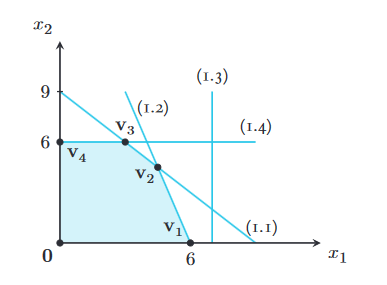
\includegraphics[width=0.5\linewidth]{linear_program.png}
    \caption[A~graphical representation of a linear program]{~A~graphical representation of a linear program~\cite{Sierksma}.}
    \label{fig:linear-problem}
\end{figure}
\\
Although for~more than two variables it would get harder to~visualize. The property of~any constraint splitting a~general hyperspace to two sub-hyperspaces still holds. Therefore, a~feasible region, if it exists, always has a~shape of~convex~polytope.\\
To~visualize the~value of~objective function over the~feasible region, we would need a~third dimension. We can either project three dimensional graph onto two dimensions, or we can draw level lines over the~two dimensional graph as~contours, connecting points in~which the~objective function has identical value. Both of~these approaches can be seen in~\autoref{fig:objective-function}
\begin{figure}[h!]
    \centering
    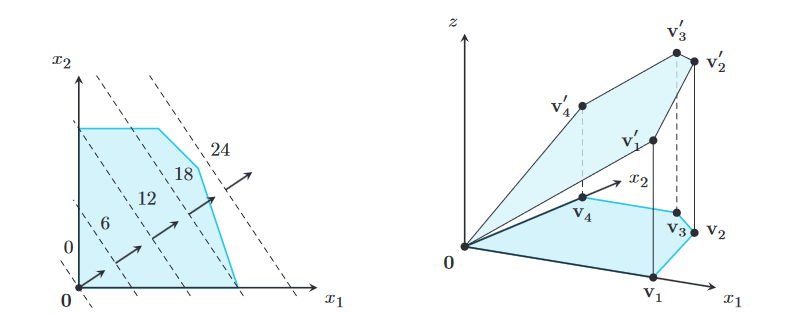
\includegraphics[width=1.0\linewidth]{objective-function.png}
    \caption[A visualization of the objective function]{A visualization of the objective function~\cite{Sierksma}.}
    \label{fig:objective-function}
\end{figure} \\
As~we can see from these visualizations, the maximal value of~the~objective function is achieved in point marked in~the~previous figures as~$v_2$, which is~the~intersection of~lines\\ ${3x_1 + x_2 = 18}$~and~${x_1 + x_2 = 9}$. This intersection can be evaluated as~$[4.5, 4.5]$, meaning that the~optimal solution of~this linear problem is~${x_1 = 4.5,\,x_2 = 4.5}$, with~value of~22.5.
\subsection{Simplex Algorithm}
\label{subsubsec:Simplex algorithm}
Description of~the~simplex algorithm can be simplified as follows: Start in one of the~vertices (points, in which the~constraints intersect, marked as~$v_i$ in~previous figures) and~then travel by~edges to~a~neighbouring vertex, in which the~value of~objective function increases (or~decreases). More detailed description is available in~the~cited monography~\cite{Sierksma}. It is good to~note that over the~years the~algorithm itself had many modifications, with~this being the~general idea that stood the~same.\\
In~this example, we might for example start in~vertex marked as~$v_1$, which has a~neighbouring vertex $v_2$, in~which the~value of~objective function is higher. Therefore we travel to~vertex~$v_2$. With all neighbours of~$v_2$ having a~lower value, we finish the~run of~algorithm. Since the~object is convex, we can safely say that we have found the~global maximum.
\section{Integer Linear Programming}
A~special case of~linear programming is the~\emph{integer~linear~programming}. In~this special case, we require some~(or~all) of~the~decision variables to~be integers, instead of~real numbers. As we have discussed, the~linear programming is solvable in polynomial time. On~the~other hand, the~integer linear programming is known to~be NP-hard already for instances where the~domain is $\{0, 1\}$ as shown in~\cite{Karp}.
On~a~positive note, integer~linear~programming is one of~the~most efficiently solvable NP-hard problems with~existing software. In~our work, we are going to~reduce many problems onto~problem of~integer~linear~programming and~use the~help of~existing solver introduced in~the~next section.
\section{Gurobi Optimization}
\textit{Gurobi optimization engine}~\cite{gurobi} is one of~the~best available solvers for linear programming, integer linear programming and~other mathematical optimization problems.
Gurobi is internally switching used algorithm, based on~the~input, and it is also able to~run the~computation in~parallel on~multiple threads.\\
It offers an interface for many programming languages, including Python, C++, and many more. We have used this solver for solving the~problem of~integer linear programming, as~the~solver is greatly optimized and~provides a~good way of~solving NP-hard problems.

\chapter{Previous Research of Sidewalk and Pedestrian Networks}
The~sidewalk networks have not been studied as~exhaustively as~the~other types of~real-world networks~(like road networks or infrastructural networks). Mainly since they do not suffer from~congestion and~overcrowding so much, compared to~the~other types of~networks. However, in~the~last years, the~attention given to~sidewalks and~generally pedestrians has risen. This is a~reflection of~promoting walking as a~mean of~transport. With the~growing attention to~sustainability and~protection of~the~planet~Earth, walking is~(and~the~trend is most likely going to~continue) becoming a~promoted mean of~transport worldwide. Therefore, modern science pays closer attention, whether cities are designed so that walking is a~sufficient alternative for~other, more pollution-heavy, means of~transport, especially personal cars. \\
However, typical main article of~research, of~most works concerned by~this topic, are not sidewalks, but rather generally \textit{pedestrian networks}. To~simplify the~difference between these two terms, pedestrian networks include sidewalks, but apart from that, they also include pedestrian crossings, residential roads or~patches of~green, which pedestrians typically use for~walking. Additionally, some sidewalks might also not be a~suitable part of~pedestrian network, if the~sidewalk is damaged or~inaccessible. \\
The~main research topics of sidewalk networks or pedestrian networks vary, however there has been no such work, measuring graph properties of sidewalk networks purely for theoretical research. On~the~other hand, there have been few studies concerned with the~similar topic, we will mention a few of them in this chapter.\\
In~\cite{Rhodas}, Rhodas~et~al. are measuring betweenness~centrality and general efficiency~of~pedestrian networks. These parameters are typically measured for~other types of~networks (as discussed earlier, road networks or infrastructure networks), as~it is an~important parameter for~identifying bottlenecks in~networks, preventing congestion. Apart from that, the~authors are giving an~attention to sidewalk coverage and~availability. Studying, whether a~pedestrian can use walking as~a~mean of transport, to~fulfill their needs, with a~special attention to~the~length of~tour they have to~take to~do so. As~it is mentioned in this~work, a~pedestrian walking on~a~sidewalk is in~constant danger of~getting involved in~an~accident. The~danger walking brings is another topic of~this work, with~a~final takeaway that future cities should minimize the~distance a~pedestrian needs to~travel. \\
The~dangers that pedestrians face while walking are also analysed in~\cite{Osama}. In this work, Osama and~Sayed are evaluating the~impacts of~pedestrian network structure on~safety of~its users. Authors are studying the~probability of~a~pedestrian being involved in~a~crash, subject to~factors, such as~continuity, linearity, coverage and~slope of~the~pedestrian network. \\
\\
\begin{samepage}
Our work varies in~two main points. First of~all, we are interested solely in~the~sidewalk networks, rather than the~pedestrian networks, as~our motivation is to~create a~realistic sidewalk network generator for 3D~model generation\footnote{Therefore, for example pedestrian crossings can not be generated together with the~sidewalks, as they are visually completely different.}. Secondly, we are studying the~sidewealk networks in a~much more theoretical way, as~we want to give an~insight to~this topic purely from~the~perspective of~discrete mathematics and~graph theory. \\
\end{samepage}
Many works studying sidewalk or pedestrian networks remark that obtaining datasets for~studying these networks is a~considerably harder task, compared to~obtaining similar data for other types of~real-world networks. Stating that this is once again due to the~fact that sidewalk network analysis has not been deemed as important as analysis of the other types of networks. We certainly can concur with this notion. In fact, availability of~road networks being significantly higher than the~availability of~sidewalk networks, is the~main motivation for designing an~algorithm that could generate a~realistic sidewalk network from road network and building outlines.
\chapter{Obtaining the Data}
In this chapter, we discuss the~process of~obtaining the~data of~sidewalk networks. We start by~describing data formats. Then we introduce the~source of~our data. And we finish this chapter with the~description of~the~process of~collecting and~serializing the~data.
\section{Data Formats}
With growing number of~applications operating with data, the need for unification of~\textit{data~formats} used has risen. In~this section we are going to~introduce few modern data formats used by~computational programs, web services, desktop applications and other software.
\subsection{XML}
\label{subsec:XML}
\textit{XML}\footnote{eXtensible Markup Language} is a~markup language defining a~structure of~documents for storing generally any type of~data. \\
XML document consists of~elements. Start of~an~element is marked with~the~\textit{opening~tag} and~the~end is marked with the~\textit{closing~tag}. The~opening tag consists of~the~opening angular bracket, name of~the~element, additional non-mandatory attributes and the~closing angular bracket. The~closing tag contains the~opening angular bracket, backslash, the~name of~the~element and~the~closing angular bracket. The~names in~the~opening and~closing tags must match. \\
An~element can contain other elements in~its body~(space between the~opening and~closing tags), thus creating the structure of~the~document. An~XML document starts with~the~version and~encoding specification, followed by~root element, which contains all other elements in~the~document.
An~example of XML document can be seen in~\autoref{cs:xml-example}.
\begin{listing}[ht!]
\begin{minted}{xml}
<?xml version="1.0" encoding ="UTF-8" ?>
<bookstore>
    <book category="fiction">
        <title>Harry Potter and the Sorcerer's Stone</title>
        <author>J.K. Rowling</author>
        <year>1997</year>
        <price>20.00</price>
    </book>
    <book category="non-fiction">
        <title>On the Origin of Species</title>
        <author>Charles Darwin</author>
        <year>1859</year>
        <price>15.00</price>
    </book>
</bookstore>
\end{minted}
\caption{An example of XML document.}
\label{cs:xml-example}
\end{listing}
XML aims to be a human-readable, self-descriptive format to be used for data exchange, configuration files and other use cases.~\cite{xml:w3c}


\subsection{JSON}
\textit{JSON}\footnote{JavaScript Object Notation} is another data format for~representing data of~any kind. It was designed to~be more light-weight, more human-readable and easier for parsing and generating by~computers than other data formats. \\
The JSON format consists of objects. An~object is enclosed by curly brackets. The~object contains key-value pairs, with key being the~name of~an~attribute, enclosed by quotation marks. The value may be in a~string format (enclosed by quotation marks), array format (enclosed by sharp brackets, containing any number of objects or primitive values), number format or boolean format. The individual key-value pairs are separated by a comma and between the key and the value in a pair, there is a colon.
An example of JSON representing the same entities as the XML document from the~previous section can be seen in~\autoref{cs:json-example}~\cite{json}
\begin{listing}[ht!]
    \begin{minted}{json}
{
  "bookstore": {
    "books": [
      {
        "category": "fiction",
        "title": "Harry Potter and the Sorcerer's Stone",
        "author": "J.K. Rowling",
        "year": 1997,
        "price": 20.00
      },
      {
        "category": "non-fiction",
        "title": "On the Origin of Species",
        "author": "Charles Darwin",
        "year": 1859,
        "price": 15.00
      }
    ]
  }
}
\end{minted}
\caption{An example of JSON representation.}
\label{cs:json-example}
\end{listing}

\subsection{GR}
\textit{GR}\footnote{Graph format} is a format used by PACE~\cite{PACE} for encoding of~undirected graphs, as defined in~\autoref{sec:Graph}. This format is used for annual competitions focused on implementing the most efficient algorithms for computationally complex problems. 
This format is designed mainly with~efficiency in~mind and~it is supposed to~be very quickly and~easily readable by~a~computer.\\
The~description of~the~graph starts with a~\textit{p-line}. This line starts with a~letter~\textit{p} followed by~an~abbreviation of~the~problem, for~which the dataset was defined\footnote{For example \textit{tw} as treewidth.}. Additionally p-line includes two numbers. The~first number represents the~number of~vertices, and~the~second~one represents the~number of~edges. p-line is followed by~a~list of~edges, each line represents one edge given by~a~pair of~vertices split by~a~single space. The vertices are being implicitly represented as~natural numbers from~1 to~number of~vertices. An~example of~this~graph encoding can be seen in~\autoref{cs:gr}, where we can see Petersen~graph~(as defined in \autoref{subsec:petersen}) encoded into~GR.
\begin{listing}
\begin{minted}{text}
p tw 10 15 
1 2
1 5
1 6
2 3
2 7
3 4
3 8
4 5
4 9
5 10
6 8
6 9
7 9
7 10
8 10
\end{minted}
\caption{GR representation of Petersen graph}
\label{cs:gr}
\end{listing}

\section{OpenStreetMap}
\textit{OpenStreetMap}\footnote{Abbreviated as OSM, also incorrectly called Open Street Map or Open Street Maps.} is a~free, collaborative and~open map~of~planet~Earth built by volunteers. Apart from the map, OSM makes publicly available data it uses for creation of the map. An~example of~the~map can be seen in~\autoref{fig:osm}. \\ 
The publicly available data from OpenStreetMap are widely used for~building other projects\footnote{One of them being the VBS Blue.}, since~the~OSM provides a~rich API\footnote{Application Programming Interface} for retrieving of this data. \cite{osm-foundation-about, ramm}
\\
\\
\\
\\
\begin{figure}[h]
    \centering
    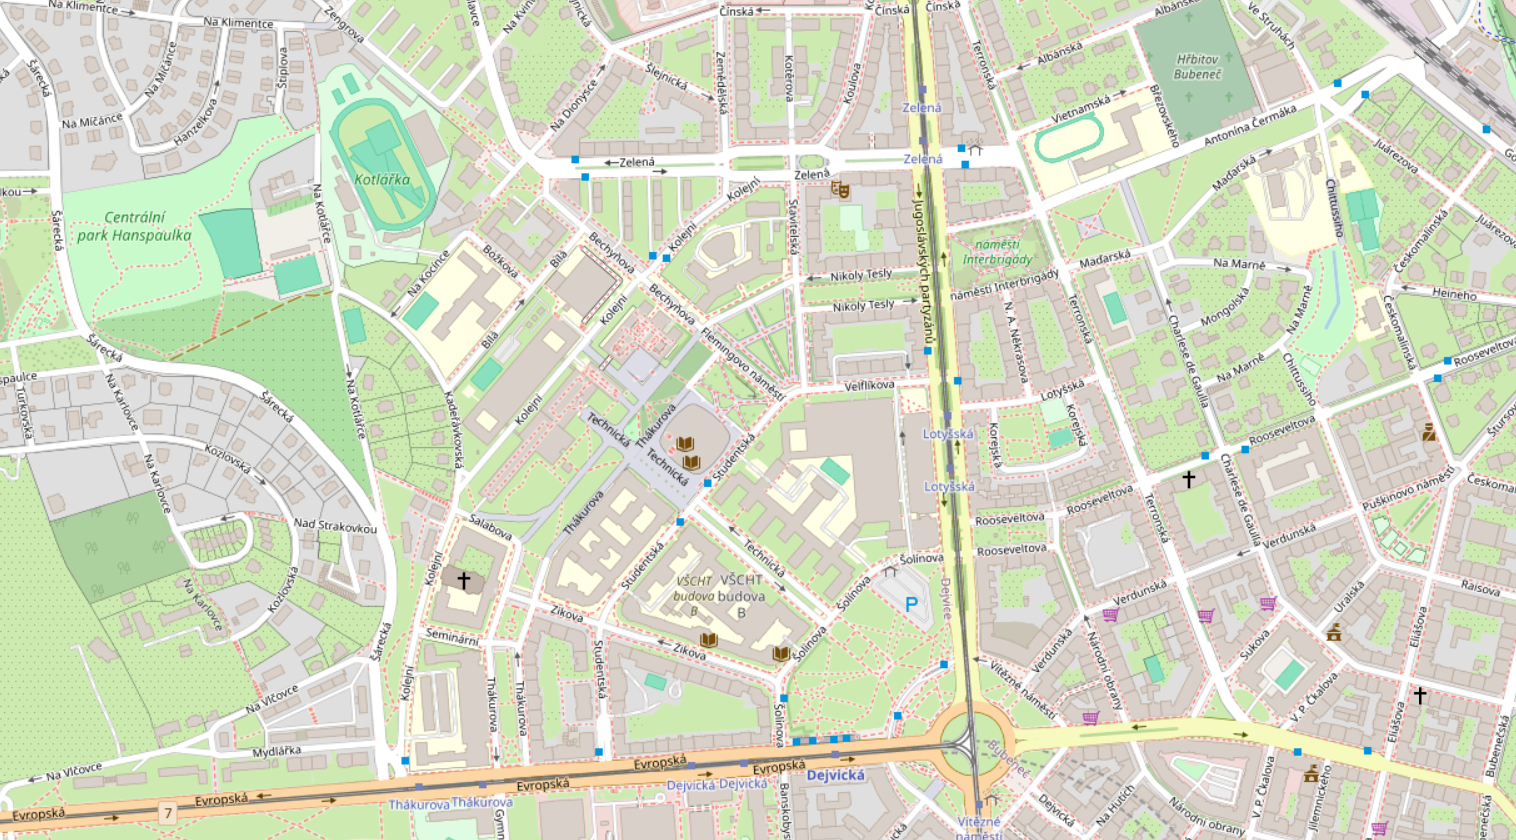
\includegraphics[width=1\linewidth]{osm.png}
    \caption[A map from OpenStreetMap project]{A map from OpenStreetMap project~\cite{osm-foundation-1}.}
    \label{fig:osm}
\end{figure}

\subsection{History}
The~OpenStreetMap project was founded in~2004 by Steve~Coast, initially focusing on~mapping of~the~United~Kingdom. In~2006, \textit{OpenStreetMap~Foundation} was established to~promote, support and~protect the~project. However OpenStreetMap~Foundation does not own the~data, as~nobody owning the data is the~main idea behind this~project. In~the~same year, Yahoo let its aerial photography to~be a~base for~OpenStreetMap, which enabled more contributors to~get involved, benefiting the~project massively. \\
The ways for importing and exporting the~data only continued to~grow. For~example, in~year~2008, the~data became exportable to~portable GPS\footnote{Global Positioning System}~devices. Nowadays, OSM is a~very unique project, which distributes quality geographical data for~free and~various usage. However, it is good to~note that the amount of~detail varies significantly depending on~the region.

\subsection{Format}
OpenStreetMap defines its own data format for data available via its API. This format is called \textit{OSM~XML} and~it is based on~XML.\\
An~OSM~XML file begins with the version of~OSM~API, followed by~bounding box~(described in the~geographic coordinate system). The~main part of~the~document consists of~list of~\textit{nodes}, list of~\textit{ways} and~list of~\textit{relations}. These terms are defined in~following subsections.
\subsubsection{Tag}
A \textit{tag} is a singular property of a real-world object represented by a~key word pair.
An~example of~a~tag can be seen in~\autoref{cs:tag-example}.
\begin{listing}[ht!]
\begin{minted}{xml}
<tag k="colour" v="brown"/>
\end{minted}
\caption[An example of a single tag from OSM]{An example of a single tag from OSM, response from~OSM~API to~GET~/api/0.6/node/2905214181, modified.}
\label{cs:tag-example}
\end{listing}
\subsubsection{Node}
A \textit{node} is a~representation of~a~single point feature, or more commonly it is a part of a \textit{way}, another OSM entity, defined in the~next section. \\
Every node contains its ID\footnote{ID stands for identificator}, latitude and longitude. Additionally, a~node can include any number of~tags (with no tags also being a~possibility), describing better what kind of a~real-world feature the~node represents. \\ 
An example of a node from OSM representing a bench can be seen in \autoref{cs:node-example}.
\begin{listing}[ht!]
\begin{minted}{xml}
<osm 
    version="0.6" 
    generator="CGImap 0.9.2 (1123753 spike-07.openstreetmap.org)"
    copyright="OpenStreetMap and contributors"
    attribution="http://www.openstreetmap.org/copyright" 
    license="http://opendatacommons.org/licenses/odbl/1-0/">
<node
    id="2905214181"
    visible="true"
    version="3"
    changeset="95334039"
    timestamp="2020-12-05T13:28:55Z"
    user="koldas"
    uid="6383771"
    lat="50.1034230"
    lon="14.3903959">
<tag k="amenity" v="bench"/>
<tag k="backrest" v="no"/>
<tag k="colour" v="brown"/>
<tag k="material" v="wood"/>
</node>
</osm>    
\end{minted}
\caption[An example of a single node feature from OpenStreetMap]{An example of a single node feature from OpenStreetMap, a~response from~OSM~API to~GET~/api/0.6/node/2905214181, reformatted.}
\label{cs:node-example}
\end{listing}
\subsubsection{Way}
\label{subsec:Way}
A \textit{way} is an~ordered sequence of~nodes. A way is used for~representation of~linear features~(like roads or~sidewalks) or~outlines of~areal features~(like building outlines or state borders). Apart from nodes, it can contain any number of~tags better describing the~real-world feature. An~example of a~way from~OSM representing a~residential road can be seen in~\autoref{cs:way-example}
\begin{listing}[ht!]
\begin{minted}{xml}
<osm
    version="0.6"
    generator="CGImap 0.9.2 (1214374 spike-07.openstreetmap.org)"
    copyright="OpenStreetMap and contributors"
    attribution="http://www.openstreetmap.org/copyright"
    license="http://opendatacommons.org/licenses/odbl/1-0/">
<way 
    id="8588965"
    visible="true"
    version="21"
    changeset="143633267"
    timestamp="2023-11-04T23:21:02Z"
    user="Martin2035"
    uid="6588887">
    <nd ref="683826"/>
    <nd ref="1244162315"/>
    <nd ref="60953383"/>
    <nd ref="60953384"/>
    <nd ref="331441551"/>
    <nd ref="683828"/>
    <tag k="bicycle" v="yes"/>
    <tag k="covered" v="no"/>
    <tag k="highway" v="residential"/>
    <tag k="lanes" v="1"/>
    <tag k="lit" v="yes"/>
</way>
</osm>
\end{minted}
\caption[An example of a way feature from OpenStreetMap]{An example of a way feature from OpenStreetMap, a response from OSM API to~GET~/api/0.6/way/8588965, reformatted, modified.}
\label{cs:way-example}
\end{listing}
\subsubsection{Relation}
A \textit{relation} is an~ordered sequence of~nodes and~ways which are connected together, typically in~a~more abstract way. Relations are typically used for~modeling of~cities, states and~other regions. Relations can optionally include tags, just like the~other entities. An~example of~a~relation from~OSM can be seen in~\autoref{cs:relation-example}
\begin{listing}
\begin{minted}{xml}
<osm
    version="0.6"
    generator="CGImap 0.9.2 (3191307 spike-07.openstreetmap.org)"
    copyright="OpenStreetMap and contributors"
    attribution="http://www.openstreetmap.org/copyright"
    license="http://opendatacommons.org/licenses/odbl/1-0/">
<relation
    id="428868"
    visible="true"
    version="16"
    changeset="143023364"
    timestamp="2023-10-23T15:16:14Z"
    user="StenSoft" uid="255936">
<member type="node" ref="297896636" role="admin_centre"/>
<member type="way" ref="181639516" role="outer"/>
<member type="way" ref="181639512" role="outer"/>
<member type="way" ref="181639509" role="outer"/>
<member type="way" ref="181639506" role="outer"/>
<member type="way" ref="512311736" role="outer"/>
<member type="way" ref="181639502" role="outer"/>
<member type="way" ref="181639496" role="outer"/>
<member type="way" ref="180740868" role="outer"/>
<member type="way" ref="577535890" role="outer"/>
<tag k="admin_level" v="10"/>
<tag k="boundary" v="administrative"/>
<tag k="name" v="Dejvice"/>
</relation>
</osm>
\end{minted}
\caption[An example of a relation from OpenStreetMap]{An example of a relation from OpenStreetMap, response from OSM API to~GET~/api/0.6/relation/428868, reformatted,}
\label{cs:relation-example}
\end{listing}
\subsection{APIs}
OpenStreetMap specifies two~different APIs, both with different use-cases. The~first one is the~classical modern API enabling both reading and writing of~raw OSM~data. Apart from that, OSM also provides a~read-only API called \textit{Overpass~API}. Overpass~API does not enable modification of~data, its purpose is only to~fetch the~data. Overpass~API is ready for handling big chunks of~data and~defines its own querying language. This language more resembles a~scripting language, rather than a~classical query language. It provides concepts better known from programming and~scripting languages, like cycles or~conditional jumps. The~main purpose of~this language is to~give user a~simple way for~obtaining and~filtering the~data, as~the~amount of~OSM data in certain parts of~the~world is humongous. Therefore, if user is interested in~specific data for~their application, they can easily filter unwanted data on~OSM server side.
\subsection{OSMnx}
Most modern programming languages have multiple dedicated libraries or~packages for communication with~OSM~Overpass~API. One of~them being the~\textit{OSMnx}~\cite{osmnx}, which is a~Python package specialized for~obtaining network data from~OSM. OSMnx uses data representations compatible with another Python package \textit{NetworkX}~\cite{networkx}~(Python package for studying of networks, mostly from~the~perspective of~graph theory).
\section{Collecting and Serializing the Data}
As a~source of~the~data we have used the~OpenStreetMap. Choosing OpenStreetMap was one of~the~most straight-forward decisions we have made, as~the~whole existing project of~VBS~Blue\, uses OSM as~its source data for~various features~(including road networks or~building outlines, which would be the~input data of~the~future potential algorithm). \\
It should be noted that there are not many better alternatives. As~we have discussed in~previous chapter, obtaining sidewalk data is a fairly more challenging task than obtaining, for example, road network data. \\
\subsection{Analysed Locations of the World}
As we have mentioned in the~previous section covering the~OpenStreetMap project, the~level of~detail in~OpenStreetMap highly depends on~the~location we choose to~study. Non-surprisingly, the~level of~detail is at~its highest in~the~most developed or~the~most culturally significant parts of~the~world. \\
We have used the~assistance of~a~community managed website \cite{bestofosm}, which summarizes the~most well-mapped placed in~the~OSM~project. Although, we had to~ensure ourselves that the destinations include the~sidewalk data, as~they are often not present, even in~places, marked by~this site as~the "Best of OSM". \\
We have tried to~make the~datasets more diverse, as the~city design naturally varies over different nations and~cultures. Unfortunately, there is only a~very few data available outside of~Europe and~the~United~States. On~the~other hand, the~city design in~Europe is very different compared to the~American one. \\
In the~end, we have settled for~the~following destinations of~the~world:
\begin{samepage}
\begin{itemize}
    \item Černý Most, Prague, Czech Republic;
    \item Cēsis, Latvia;
    \item College Park, Maryland, United States of America;
    \item Dejvice, Prague, Czech Republic;
    \item Grenoble, France;
    \item Helsinki, Finland;
    \item Raleigh, North Carolina, United States of America;
    \item Donostia-San Sebastián, Spain\footnote{Official name of Donostia-San Sebastián is a bilingual combination of Basque and Spanish name of the city (both meaning Saint Sebastian), in this work we will refer to this city as San Sebastián, as it is a name more commonly used outside of the Basque area.};
    \item Santa Cruz, California, United States of America.
\end{itemize}
\end{samepage}
%Maybe introduce the locations
\subsection{Usage of OSMnx Package}
When we selected the~locations, obtaining their sidewalk data from~OSM was not a~difficult task. We have taken all features having a~value of~tag \texttt{highway} set to~\texttt{footway}, \texttt{path} or~\texttt{steps}; or~a~value of~tag~\texttt{foot} set to~\texttt{designated} or~\texttt{yes}. \\
With the~help of~Python package OSMnx~\cite{osmnx}, we have been able to~acquire the~data using just a~few lines of~code, which can be seen listed in~\autoref{cs:osm-data}.\\
This code snippet generates an outcome as in \autoref{fig:dejvice}.
It can be seen,that the~data obtained from~OSM include more information than we need, such as~the~location of~the~vertices or~shapes of~the~edges. Since we were interested solely in~vertices and~edges connecting them, we have simplified the~data before serializing, forgetting the~unnecessary information. \\
We have serialized the~obtained data into~JSON and~GR~formats. \\
The~JSON format is~a good general representation of~any data. Therefore exporting the~data to~a~JSON was the~first thing we have done. We have decided to~use the~following JSON representation. The~object of~graph includes two lists, called "vertices" and "edges". The~list of~vertices is an~unordered list of~unique numbers. These numbers are OSM~IDs of~OSM nodes represented by~these vertices. The list of~edges is a~list of~lists of~length two~(for~simplicity, we will call these lists \textit{pairs}). Each pair represents an~edge in~the~graph. Naturally, such pair represents an~edge between the~two vertices it contains. \\
For exporting data into~JSON, Python is already providing a~library without any additional package, therefore the~export was a~simple task. \\
Additionally, we have decided to~export the~data into~the GR~format, as~many solvers used for identifying the~structural properties of~the~networks accept input in~this format. We have done the~conversion to~GR format ourselves. The main difference between the~chosen JSON representation and~the~GR~format is that GR~format implicitly represents the~vertices as~natural numbers between 1 and the~number of~vertices, whereas our JSON~format uses the~OSM~IDs for~vertex representation.
\begin{listing}
    \begin{minted}{python}
#!/bin/env python3

from osmnx import graph_from_place, plot_graph as ox_plot_graph, project_graph
import networkx as nx
import matplotlib.pyplot as plt

def get_osm_graph(place_name : str) -> nx.MultiDiGraph:
    """
        Fetches data of sidewalks from place given by place_name
    """
    custom_filters = ['["highway"~"footway|path|steps"]','["foot"~"yes|designated"]']
    graph_parts = [graph_from_place(place_name, network_type='all', retain_all=True, simplify=True, custom_filter=custom_filter)
                    for custom_filter in custom_filters]
    
    return nx.compose_all(graph_parts)

def visualize_osm_data(graph : nx.MultiDiGraph):
    """
        Visualization of OSM data
    """ 
    ox_plot_graph(project_graph(graph))
    plt.show()  
  
def main():
    place_name = "Dejvice, Prague, Czechia"
    osm_graph : nx.MultiDiGraph = get_osm_graph(place_name)
    visualize_osm_data(osm_graph)

if __name__ == "__main__":
    main()
    \end{minted}
    \caption{Python script exporting and visualizing the sidewalk data from OSM.}
    \label{cs:osm-data}
\end{listing}
\begin{figure}
    \centering
    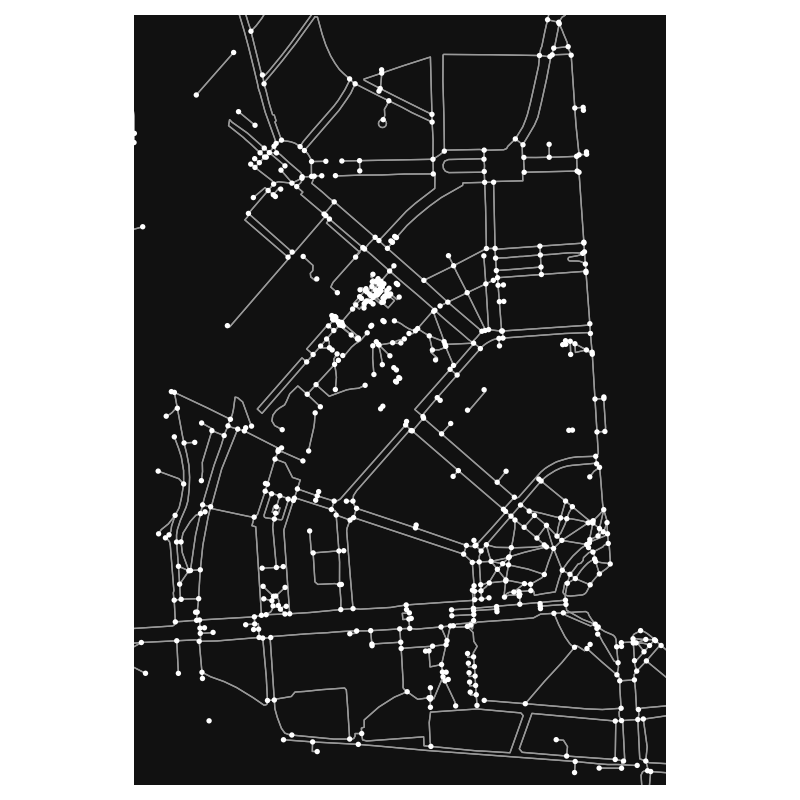
\includegraphics[width=1.0\linewidth]{dejvice.png}
    \caption{A visualization of the data obtained from OSM for Dejvice, Prague, Czech Republic.}
    \label{fig:dejvice}
\end{figure}
\chapter{Graph Properties Measurement and Evaluation}
The~main part of~our research was the~analysis of~graph properties of~the~real-world sidewalk networks. In~this chapter, we will go through the~process of~measuring properties, describing challenges it brought, and~how we coped with~them. We will also describe the~reason, why we selected these particular properties for measuring, and~discuss our results, stating the~main takeaways for the~development of~the~sidewalk network generating algorithm.
\section{Feedback Edge Set Number}
The~first property we measured was the~\textit{feedback~edge~set~number} of~the graphs, as~defined in~\autoref{subsubsec:fesn}.
\subsection{Motivation}
The~feedback~edge~set~number is a~property that could help us massively in~creation of~the~algorithm for~sidewalk generation. Our first idea for designing such algorithm is to~identify vertices~(how should the~vertices be identified is yet undisclosed) and~continue by finding a~minimal spanning tree\footnote{Minimal in its length.}. At~that point we would start adding edges to~make the~network look more realistic. How many edges we should add can be answered by~this parameter.
\subsection{Measurement}
Measuring value of~this property was a~surmountable task. Finding feedback edge set number is a~problem known to be solvable in~polynomial time. The~idea of~the~polynomial algorithm is fairly simple. Spanning trees~(or~forests) are maximal acyclic subgraphs. Therefore to~find the~feedback~edge~set~number of~a~given graph, we take the~difference between the~number of~its edges and~the~number of~edges in~any of~its spanning trees (or forests).~\cite{Beineke} \\
For any connected graph $G = (V, E)$ and~its spanning tree $G_T = (V, E_T)$, the~feedback~edge~set~number is equal to~$|E| - |E_T|$. The problem can be simplified further, when we realize that the~number of~edges in a~spanning tree, can be identified just from the~number of~vertices of~the~graph. Using one of~the~alternative definitions of~a~tree: Graph $G = (V, E)$ is a~tree $\iff$ it is connected and~$|E| = |V| - 1$, we can conclude that we can replace $|E_T|$ in~the~expression and get a~simple way to~calculate~feedback~edge~set~number for a~connected graph as~$|E| - |V| + 1$.\\
Furthermore, we can handle disconnected graphs in~a~similar way, using this expression for~all of~its connected components. For any graph $G$ and its maximal connected components:\\ ${G_1 = (V_1, E_1),\, G_2 = (V_2, E_2),\,\dots,\,G_k = (V_k, E_k)}$ such $\bigcup_{i=1}^{k} G_i = G$, we can calculate the~feedback~edge~set~number as~$\sum_{i=1}^{k} |E_i| - |V_i| + 1$. We can split this sum into separate sums as follows $\sum_{i=1}^{k} |E_i| - \sum_{i=1}^{k} |V_i| + \sum_{i=1}^{k} 1$. And since all connected components are disjoint and~add up to~the~whole graph $G$, we can rewrite this as~follows: $|E| - |V| + k$, where $k$ is the~number of~connected components of~$G$. Since a~connected graph will have $k$ equal to~1, this expression can be actually applied on~all graphs, regardless of~whether they are connected or~not. This is the~expression we used to~identify the~feedback~edge set~number of~the~sidewalk~networks.
\subsection{Results}
First, we show our results for~all datasets in~\autoref{tab:fesn}. In~this~table, we abbreviate feedback~edge~set~number as~FESN and feedback~edge~set as~FES.
\begin{table}[h!]
\centering
\caption[Measured values of feedback edge set number]{~Measured values of feedback edge set number.}\label{tab:fesn}
\begin{tabular}{l|c|c|c|c}
	\textbf{Dataset}		& $\|\mathbf{V}\|$		& $\|\mathbf{E}\|$& \textbf{FESN}   & \textbf{Relative size of FES}\tabularnewline \hline \hline
 	Černý Most, PRG, CZE & 1\,553	& 1\,893 & 377 & 24.87\,\%\tabularnewline \hline
 	Cēsis, LAT	& 1\,122	& 1\,244	& 245 & 24.52\,\%	\tabularnewline \hline
 	College Park, MD, USA & 5\,110 & 6\,392 & 1\,534 & 31.58\,\%	\tabularnewline \hline
 	Dejvice, PRG, CZE & 1\,675 & 1\,907 & 372 & 24.23\,\%	\tabularnewline \hline
 	Grenoble, FRA & 9\,647 & 11\,688 & 2\,711 & 30.20\,\%	\tabularnewline \hline
 	Helsinki, FIN & 115\,318 & 123\,291 & 18\,483 & 17.64\,\%	\tabularnewline \hline
 	Karlín, PRG, CZE & 1\,070 & 1\,364 & 345 & 33.86\,\%	\tabularnewline \hline
 	Raleigh, NC, USA & 36\,385 & 39\,930 & 5\,667 & 16.54\,\%	\tabularnewline \hline
 	San Sebastián, ESP & 4\,782 & 4\,961 & 813 & 19.60\,\%	\tabularnewline \hline
 	Santa Cruz, CA, USA & 13\,060 & 14\,494 & 2\,710 & 23.00\,\%	\tabularnewline
\end{tabular}
\end{table}
\\
We can see that the~feedback edge~set~number differs across all datasets considerably. It came as~no surprise; rather, it aligned with~our anticipatory projections, that with the~increasing number of~edges, the~size of minimal feedback~edge~set will also grow. \\ 
Therefore, apart from feedback edge set number, we have also measured the~relative size of~the~minimal feedback~edge~set. The~relative size of~feedback~edge~set expresses, how big is the~feedback~edge set compared to~the~rest of~edges. To~be more specific, the~exact formula used for calculation is~$\frac{f}{\|E\| - f}$, where~$f$ is the~value of~the~feedback~edge~set~number. We can see that this number does not differ too dramatically. \\
We are interested in this ratio, as~it gives us a~relative number of~edges we should add, after we have constructed the~spanning tree for vertices, in~the~generation algorithm. We can see that this number typically stays around 20\,\% and for bigger datasets (which are generally more trustworthy, as~they do not contain that many false endpoints, where the~network is ended by the end of the~dataset, rather than the~actual end of the~sidewalk), it gets even lower.
\section{Feedback Vertex Set Number}
After we have successfully measured the~feedback~edge~set number, we continued with~the~\textit{feedback~vertex~set~number},  a~property, which we have defined in~\autoref{subsubsec:FeedbackVertexSetNumber}.
\subsection{Motivation}
We were interested in~the~feedback~vertex~set~number, as~it is a~parameter that could tell us whether the~selection of~vertices in~the~algorithm is structurally correct. Additionally, since deciding the~feedback~vertex~set~number is definitely a~non-trivial task, with the~problem being NP-hard, our results can provide a~rough estimation for any sidewalk network, without the~need of~the~computationally intense calculation of~the~parameter.
\subsection{Measurment}
As we have mentioned, deciding the~value of the~feedback~vertex~set~number is a~problem belonging to~the~NP-hard class. Therefore, for calculation of~this property, we have used existing solvers. Despite that, for the biggest datasets, we can still only provide boundaries of~the~value, rather than the~exact value, which proved to~be too difficult to~measure in~some cases.
\subsubsection{Exact Value and Upper Bound}
For~calculation of this property, we have used a~solver developed by~Iwata~and~Imanishi~\cite{Iwata1, Iwata2}, as~a~part of~PACE challenge~2016. \\
This solver gives an~upper bound and~incrementally improves it, until it reaches an~optimum, at~which point it stops.\\
We were able to~obtain the~exact value of~the~feedback~vertex~set~number for few datasets. We were also able to~get an~upper bound for almost all the~datasets, apart from the~biggest ones. \\
The~specification of~the~challenge mentions that the~solvers were tested against graphs with the~number of~vertices ranging from 30~to~20\,000, therefore it does not come as a~surprise that the~dataset of~Helsinki (with more than 100\,000 vertices), does not get any upper bound calculated. \\
What was more surprising, was definitely the~solver achieving the best performance on~the~dataset representing the~city of~San~Sebastián. This dataset belongs among our datasets to~the~ones with the~medium size\footnote{In terms of number of vertices and edges.}, so it was rather an~unexpected outcome. At this point, we were not able to~tell the~reason, why the~solver computed the~feedback vertex~set~number of~this dataset so swiftly. An~answer for this question we got, after we have measured the~treewidth of~the~datasets. We will discuss this topic in-detail in~the~following section.
\subsubsection{Lower Bound}
We have also measured the~lower bound, although it does not carry as~much value as~the~upper bound. On~the~other hand, we were able to~measure the~lower bound for all of~the~datasets, including the~biggest ones. \\
For the~calculation of~the~lower bound, we have used the~integer linear programming. First, we used the~NetworkX library~\cite{networkx} to identify all cycles in~a~graph, and then we used the Gurobi solver~\cite{gurobi} to find a~minimal hitting set of the~cycles. Formal description of~the~mathematical model used for the~calculation of this property is: \\
Let $F$ be a~set of cycles contained in~$G = (V, E)$, let there be a~variable~$x_v$ for every vertex $v \in V$, set to 1 if the~vertex~$v$ is present in the~feedback vertex set; else set to~0. Minimize $\sum_{v \in V} x_v$ subject to $\forall\,C \in F:\sum_{v \in C} x_v \geq 1$. \\
This description corresponds to the second definition given in \autoref{subsubsec:FeedbackVertexSetNumber}. \\
However, finding all cycles in a graph, is also a~computationally very complex task~(with~all cycles found we would be easily able to~decide, whether one of~them is a~\textit{Hamiltonian cycle}\footnote{Hamiltonian cycle is a~cycle containing all vertices of a~graph.}, this decision problem is known to be NP-hard~\cite{Karp}). However we would only need that for the~exact computation. Since we wanted to provide a~lower bound, we have used a~length boundary for cycles~(namely 9), giving us an~incomplete set of~cycles in acceptable time. We have then found a~minimal subset of~vertices that covers this~subset of~cycles. Such subset of~vertices will surely be smaller than the~minimal~feedback~vertex~set, therefore we got a~lower bound for the~feedback~vertex~set~number.
\subsection{Results}
Let us start once again with~the~outcome of~our measurements, which can be seen in~\autoref{tab:fvsn}. In~this~table, we abbreviate feedback~vertex~set~number as~FVSN and feedback~vertex~set as~FVS.
\begin{table}[h!]
\centering
\caption[Measured values of feedback vertex set number]{~Measured values of feedback vertex set number.}\label{tab:fvsn}
\begin{tabular}{l|c|c|c|c}
	\textbf{Dataset}		& $\|\mathbf{V}\|$		& $\|\mathbf{E}\|$& \textbf{FVSN}   & \textbf{Relative size of FVS}\tabularnewline \hline \hline
 	Černý Most, PRG, CZE & 1\,553	& 1\,893 & 146--167 & 10.38--12.05\,\%\tabularnewline \hline
 	Cēsis, LAT	& 1\,122	& 1\,244	& 110--113 & 10.87--11.20\,\%	\tabularnewline \hline
 	College Park, MD, USA & 5\,110 & 6\,392 & 571--595 & 12.58--13.18\,\%	\tabularnewline \hline
 	Dejvice, PRG, CZE & 1\,675 & 1\,907 & 173 & 11.52\,\%	\tabularnewline \hline
 	Grenoble, FRA & 9\,647 & 11\,688 & 1\,017-- & 11.78--\,\%	\tabularnewline \hline
 	Helsinki, FIN & 115\,318 & 123\,291 & 7\,842-- & 7.30--\,\%	\tabularnewline \hline
 	Karlín, PRG, CZE & 1\,070 & 1\,364 & 138--153 & 14.81--16.68\,\%	\tabularnewline \hline
 	Raleigh, NC, USA & 36\,385 & 39\,930 & 2\,472-- & 7.29--\,\%	\tabularnewline \hline
 	San Sebastián, ESP & 4\,782 & 4\,961 & 407 & 9.30\,\%	\tabularnewline \hline
 	Santa Cruz, CA, USA & 13\,060 & 14\,494 & 1\,168-- & 9.82--\,\%	\tabularnewline
\end{tabular}
\end{table}
\\
Analogously to~the~feedback~edge~set~number, the~feedback~vertex~set~number also grows with the~size of~the~graph. Therefore we have once again introduced a~relative parameter expressing the~ratio of~the~feedback~vertex~set size and~the~number of vertices. \\
This calculation uses a~slightly different formula as~opposed to~the~feedback~edge~set. We have used the~formula: $\frac{f}{\|V\|}$, where~$f$ represent the~feedback~vertex~set~number. We have switched to~this formula, since at~feedback~edge~set~number, we were interested in~how many edges we should add to~a~constructed spanning~tree~(in~the~potential algorithm for~a~sidewalk network generation). This time, however, we are rather trying to~give out a~way to~estimate feedback~vertex~set~number for~any sidewalk network, from the~number of~its vertices.\\
Judging from the~exact measurements and~boundaries, we can estimate this~ratio to be~somewhere between 8~and~15~percent.
\section{Treewidth}
\label{sec:Treewidth}
Our third measured parameter was the~parameter of~\textit{treewidth} as~defined in~\autoref{subsubsec:treewidth}.
\subsection{Motivation}
The~treewidth is a~very interesting graph property. Many graph problems are simpler for~computation, when the~input graph has a~small treewidth~\cite{Diestel}. However, deciding the~treewidth itself is an~NP-hard problem. Our measurements can provide an~interesting estimation of~the~treewidth of sidewalk networks. \\
Subsequently, we can use this property for analysis of~the~outcomes of~the~future potential algorithm, to~see whether yielded outputs are correct.
\subsection{Measurment}
Measuring the~treewidth of~a~graph is a~very extensively studied topic, since it is a~parameter of a~serious value. Therefore we have used for measurement an~existing solver developed by Tamaki~\cite{Tamaki1, Tamaki2, Tamaki3}, as~a~part of~PACE challenge~2017. \\
This solver gives a~lower bound and an~upper bound, incrementally improving both, until they meet, at which point it stops. For the~smaller datasets, we were able to~get the~exact value of~the~treewidth. For the~more sizable data sets, we were able to~obtain a~lower bound and~an~upper bound. However, for~the biggest datasets, we were able to~measure neither of the boundaries.
\subsection{Results}
The~measured values can be seen in~\autoref{tab:treewidth}. The~table does not include the~datasets of~Helsinki and~Raleigh, as we have failed to measure any values for these datasets.
\begin{table}[h!]
\centering
\caption[Measured values of treewidth]{~Measured values of treewidth.}\label{tab:treewidth}
\begin{tabular}{l|c|c|c|c}
	\textbf{Dataset}		& $\|\mathbf{V}\|$		& $\|\mathbf{E}\|$& \textbf{Treewidth}   & \textbf{$\frac{\|E\|}{\|V\|}$}\tabularnewline \hline \hline
 	Černý Most, PRG, CZE & 1\,553	& 1\,893 & 10 & 1.22\tabularnewline \hline
 	Cēsis, LAT	& 1\,122	& 1\,244	& 10 & 1.11 \tabularnewline \hline
 	College Park, MD, USA & 5\,110 & 6\,392 & 15--22 & 1.25	\tabularnewline \hline
 	Dejvice, PRG, CZE & 1\,675 & 1\,907 & 9 & 1.14	\tabularnewline \hline
 	Grenoble, FRA & 9\,647 & 11\,688 & 14--25 & 1.21 \tabularnewline \hline
 	Karlín, PRG, CZE & 1\,070 & 1\,364 & 8 & 1.27	\tabularnewline \hline
 	San Sebastián, ESP & 4\,782 & 4\,961 & 7 & 1.04 \tabularnewline \hline
 	Santa Cruz, CA, USA & 13\,060 & 14\,494 & 13--16 & 1.11 \tabularnewline
\end{tabular}
\end{table}
\\
We can see that for~the~smaller datasets the~value of~the~treewidth stays around~10. For the~larger datasets, representing more populous cities, the~value rises to~20. \\
Very interesting is~the case of~San~Sebastián. This dataset has considerably lower treewidth, than we would expect from its size. To explain this occurrence, we can notice that this graph is the~most \textit{sparse} among all the~datasets. To enumerate the~"sparsity" of~the~datasets, we have calculated a~simple parameter of~\textit{ratio of~edges and~vertices}, expressed in~the~additional column. \\
Seemingly, apart from the~size of~the~graph, the~treewidth is considerably influenced by this ratio. \\
The~low treewidth of~San~Sebastián sidewalk network had a~serious impact on~its measurements. Both feedback~vertex~set~number computation and~treewidth~computation were significantly faster for this dataset, compared to the~other datasets.
\section{Vertex Cover Number}
Another parameter we have measured was the \textit{vertex~cover~number} as~defined in~\autoref{subsubsec:VCN}. 
\subsection{Motivation}
The~vertex~cover~number is another non-trivial graph parameter we have measured, as~it could be used for~confirmation of~the~results yielded by the~algorithm. We believed that we would be able to~measure this property exactly for~all datasets, since it is known to~be easily represented via~the~integer~linear~programming.
\subsection{Measurment}
We have used the~integer~linear~programming solver Gurobi~\cite{gurobi}, as~the~vertex~cover~number is known to be solvable with~the~integer~linear~programming as~described in~\cite{Vazirani}.\\
Let there be a~binary variable~$x_v$ for each vertex $v \in V$, set to~1, if the~vertex~$v$ is present in~the~vertex cover; else set to~0. Minimize $\sum_{v \in V} x_v$ subject to: ${\forall\,\{u,\,v\}\,\in\,E:\,x_u\,+\,x_v\,\geq\,1}$.
\subsection{Results}
The~results of~the~measurements can be seen in~\autoref{tab:vcn}. In~this~table, we abbreviate vertex~cover~number as~VCN and the~vertex~cover as~VC. We have been able to exactly measure the~value of~the~vertex~cover~number for all datasets, as~we expected and~hoped.
\begin{table}[h!]
\centering
\caption[Measured values of vertex cover number]{~Measured values of vertex cover number.}\label{tab:vcn}
\begin{tabular}{l|c|c|c|c}
	\textbf{Dataset}		& $\|\mathbf{V}\|$		& $\|\mathbf{E}\|$& \textbf{VCN}   & \textbf{Relative size of VC}\tabularnewline \hline \hline
 	Černý Most, PRG, CZE & 1\,553	& 1\,893 & 764 & 49.20\,\%\tabularnewline \hline
 	Cēsis, LAT	& 1\,122	& 1\,244	& 521 & 46.43\,\% \tabularnewline \hline
 	College Park, MD, USA & 5\,110 & 6\,392 & 2\,440 & 47.75\,\%	\tabularnewline \hline
 	Dejvice, PRG, CZE & 1\,675 & 1\,907 & 790 & 47.16\,\%	\tabularnewline \hline
 	Grenoble, FRA & 9\,647 & 11\,688 & 4\,672 & 48.43\,\% \tabularnewline \hline
    Helsinki, FIN & 115\,318 & 123\,291 & 52\,824 & 45.81\,\%	\tabularnewline \hline
 	Karlín, PRG, CZE & 1\,070 & 1\,364 & 535 & 50.00\,\%	\tabularnewline \hline
 	Raleigh, NC, USA & 36\,385 & 39\,930 & 16\,576 & 45.56\,\%	\tabularnewline \hline
 	San Sebastián, ESP & 4\,782 & 4\,961 & 2\,173 & 45.44\,\%	\tabularnewline \hline
 	Santa Cruz, CA, USA & 13\,060 & 14\,494 & 6\,059 & 46.39\,\%	\tabularnewline
\end{tabular}
\end{table}
\\
The~vertex~cover~number is another graph property heavily dependent on the~graph size. However, if we once again take the~relative size, defined as~$\frac{v}{\|V\|}$, where~$v$ is the~vertex~cover~number, we get a~property that is very stable among all the~used datasets. The~relative size of~the~vertex~cover stays between 45~and~50~percent at all studied graphs.
\section{Edge Cover Number}
The~last studied property was the~\textit{edge~cover~number} as~defined in~\autoref{subsubsec:EdgeCoverNumber}
\subsection{Motivation}
The~edge~cover~number is another structural parameter known to~be computable in~polynomial time~\cite{Garey}. We have decided to~measure this parameter, so that we have another parameter to~test the~results of~the~algorithm against. However, unlike the~previous three parameters, this parameter is efficiently computable. Therefore, the~potential algorithm can calculate the~value of~its currently constructed network, while it is running, and alter its result and flow accordingly. That is not possible for~the~previous properties, as~the~designed algorithm has to~be reasonably efficient~(therefore it can not solve NP-hard problems while running).
\subsection{Measurement}
Even though this is by~far not the~optimal approach\footnote{In terms of computational complexity.}. We have described this problem with~integer~linear~programming and used the~Gurobi solver~\cite{gurobi}. Although we are technically converting a~simple problem solvable in~polynomial time, to an~NP-hard problem, which may seem like an~irrational move; it was the~fastest way to create a~solver in terms of~the~human time spent developing it. Since the~Gurobi solver is greatly optimized, we were able to~get the~results for all datasets in~few seconds nevertheless. \\
We have described the~problem in~integer~linear~programming as~follows: Let there be a~binary variable~$x_e$ for every edge $e \in E$, set to~1, if the~edge $e$ is present in~the~edge cover; else set to~0. Minimize $\sum_{e \in E} x_e$ subject to: $\forall v \in V:\;\sum_{e \in E, v \in e} x_e \geq 1$.
\subsection{Results}
The~results of our measurements can be seen in~\autoref{tab:ecn}. In~this~table, ECN stands for edge~cover~number, r.~size~of~EC stands for relative~size of~edge~cover and~r.~dist.~to~opt. stands for relative~distance~to~optimum.
\begin{table}[h!]
\centering
\caption[Measured values of edge cover number]{~Measured values of edge cover number.}\label{tab:ecn}
\begin{tabular}{l|c|c|c|c|c}
	\textbf{Dataset}		& $\|\mathbf{V}\|$		& $\|\mathbf{E}\|$& \textbf{ECN}   & \textbf{R.\ Size of EC}    & \textbf{R.\ Dist.\ to Opt.} \tabularnewline \hline \hline
 	Černý Most, PRG, CZE & 1\,553	& 1\,893 & 806 & 42.58\,\% & 1.56\,\%\tabularnewline \hline
 	Cēsis, LAT	& 1\,122	& 1\,244	& 606 & 48.71\,\% & 3.62\,\% \tabularnewline \hline
 	College Park, MD, USA & 5\,110 & 6\,392 & 2\,725 & 42.63\,\%	 & 2.66\,\%\tabularnewline \hline
 	Dejvice, PRG, CZE & 1\,675 & 1\,907 & 900 & 47.19\,\%	 & 3.28\,\%\tabularnewline \hline
 	Grenoble, FRA & 9\,647 & 11\,688 & 5\,093 & 43.57\,\%  & 2.31\,\%\tabularnewline \hline
    Helsinki, FIN & 115\,318 & 123\,291 & 63\,343 & 51.38\,\%	 & 4.61\,\%\tabularnewline \hline
 	Karlín, PRG, CZE & 1\,070 & 1\,364 & 549 & 40.25\,\%	 & 1.03\,\%\tabularnewline \hline
 	Raleigh, NC, USA & 36\,385 & 39\,930 & 19\,942 & 49.94\,\%	 & 4.38\,\%\tabularnewline \hline
 	San Sebastián, ESP & 4\,782 & 4\,961 & 2\,639 & 53.19\,\%	 & 5.00\,\%\tabularnewline \hline
 	Santa Cruz, CA, USA & 13\,060 & 14\,494 & 7\,135 & 49.23\,\%	 & 4.17\,\%\tabularnewline
\end{tabular}
\end{table}
\\
We have introduced two additional columns in~the~table. First of~them being the~relative size of~the~edge cover taken against the~set of~all edges. This column is calculated using formula~$\frac{e}{\|E\|}$, where~$e$ is the~edge~cover~number. The~second additional column is a~relative distance to~optimum. The~optimum we are referring to~is the~theoretical best edge cover of~size~$\frac{\|V\|}{2}$. The~relative distance to~the~optimum is calculated as~$\frac{e - \frac{\|V\|}{2}}{\|E\|}$, where~$e$ once again represents the~edge~cover~number. \\
The~relative size differs highly, depending on the~\textit{density} of graphs. We can notice that San~Sebastián, which had low density and~therefore a~low treewidth, has one of~the~highest relative size of~the~edge cover. \\
More interesting is the~second parameter, we can see that this parameter does not exceed 5~percent for any of~the~datasets. Therefore, we can assume that the~edge~cover~number of~a~sidewalk network should typically not exceed 50~\% of its vertices + 5~\% of its edges.
\chapter{Conclusion}
We conclude this thesis with a~final table containing all the~measured data. In this table FESN stands for feedback edge set number, FVSN stands for feedback vertex set number, TW stands for treewidth, VCN stands for vertex cover number, ECN stands for edge cover number.
\begin{table}[h!]
\centering
\caption[Concluding table]{~Measured values of all parameters.}\label{tab:all}
\begin{tabular}{l|c|c|c|c|c|c|c}
	\textbf{Dataset}		& $\|\mathbf{V}\|$		& $\|\mathbf{E}\|$& \textbf{FESN}   & \textbf{FVSN}    & \textbf{TW}  & \textbf{VCN}  &   \textbf{ECN} \tabularnewline \hline \hline
 	Černý Most, PRG, CZE & 1\,553	& 1\,893 & 377 & 146--167 & 10  &   764 &   806\tabularnewline \hline
 	Cēsis, LAT	& 1\,122	& 1\,244	& 245 & 110--113 & 10    &   521 &   606 \tabularnewline \hline
 	College Park, MD, USA & 5\,110 & 6\,392 & 1\,534 & 571--595	 & 15--22 &   2\,440    &   2\,725\tabularnewline \hline
 	Dejvice, PRG, CZE & 1\,675 & 1\,907 & 372 & 173	 & 9  &   790 &   900\tabularnewline \hline
 	Grenoble, FRA & 9\,647 & 11\,688 & 2\,711 & 1\,017--  & 14--25    &   4\,672  &   5\,093\tabularnewline \hline
    Helsinki, FIN & 115\,318 & 123\,291 & 18\,483 & 7\,842--    &    & 52\,824  &   63\,343\tabularnewline \hline
 	Karlín, PRG, CZE & 1\,070 & 1\,364 & 345 & 138--153 & 8   &   535 &   549\tabularnewline \hline
 	Raleigh, NC, USA & 36\,385 & 39\,930 & 5\,667 & 2\,472--	& & 16\,576  &   19\,942\tabularnewline \hline
 	San Sebastián, ESP & 4\,782 & 4\,961 & 813 & 407	 & 7 &   2\,173  &   2\,639\tabularnewline \hline
 	Santa Cruz, CA, USA & 13\,060 & 14\,494 & 2\,710 & 1\,168--   &   13--16  &   6\,059	 & 7\,135\tabularnewline
\end{tabular}
\end{table}
\\
The~main takeaways of~our research can be summarized as~follows:
\begin{itemize}
    \item when holding a~minimum spanning tree or a~minimum spanning forest of~a~graph, we should add 15--25~\% of~edges to~create a~realistic sidewalk network;
    \item the~edge~cover~number of~a~realistic sidewalk network should not exceed 50~\% of its vertices and 5~\% of its~edges;
    \item the~minimal~vertex~cover of~a~realistic sidewalk network should contain between 45~and~50~percent of~its vertices;
    \item the~treewidth of~a~realistic sidewalk network typically stays around~10 for smaller cities or neighbourhoods of larger cities, and it stays around 20 for medium sized cities;
    \item the~minimal feedback~vertex~set of~a~realistic sidewalk network should contain between 8~and~15~percent of its vertices. 
\end{itemize}
The most natural continuation of this thesis should be the development of the algorithm for sidewalk generation, towards which this thesis has made its research. \\
Additionally, it would be very interesting to~obtain the~sidewalk network data for~other parts of~the~world~(Africa, Asia, \dots) and~measure the~values of the properties we have measured. We unfortunately could not have included these parts of~the~world because of~the~lack of~data available. It would be fascinating to~discover, whether there exists a~significant difference in~the~city design, based on~the~cultural diversity of~people around the~world. \\
Should there be an~improvement in~computation speed of~modern computers, or discoveries in~computer science of~better algorithms for calculating graph properties, it would be tempting to~remeasure the~values of~feedback~vertex~set~number or treewidth, we failed to measure exactly. \\
Also there are many more alluring graph properties to~analyse like distance~to~disjoint~stars, twinwidth, domination~numbers or maximum~independent~set~size; to name a few.
 % include `text.tex' from `text/' subdirectory

\appendix\appendixinit % do not remove these two commands

\backmatter % do not remove this command

\printbibliography % print out the BibLaTeX-generated bibliography list

\include{text/medium} % include `medium.tex' from `text/' subdirectory

\end{document}
